% This template of Ph.D./Master manuscripts was created and customized by Prof. Kamel GUESMI from the University of Djelfa (Algeria) on 09/2022. It's Free Use License for everyone. Just make an invocation for him. May Allah bless you.  
\documentclass[12pt]{report}
\usepackage[french,english]{babel}
\usepackage[T1]{fontenc}
\usepackage[utf8]{inputenc}
%\usepackage{times}
\usepackage[pdftex]{hyperref}
\usepackage{graphicx}
\usepackage[top=2cm,bottom=2cm,left=3cm,right=2cm]{geometry}
\usepackage{caption}
\usepackage{fancyhdr}
\usepackage{amsmath} 
\usepackage{textcomp}
\usepackage{pdfpages}
%\usepackage{subfig}
\usepackage{subcaption}
\usepackage{pdflscape}
\usepackage{pdfpages}
\usepackage{float}
\usepackage{multirow}
\usepackage[nottoc]{tocbibind}
\usepackage{afterpage}
\usepackage{tikz, lipsum,lmodern}
\usepackage{calligra,frcursive,xcolor}
\usepackage{pifont}
\usepackage[most]{tcolorbox}
\usepackage{fancyvrb}
\usepackage{array}
\usepackage{tabularx}
\usepackage{multirow}
\usepackage{pgfplots}
\linespread{1.3} 
\renewcommand{\footrulewidth }{0.3pt}
\hypersetup{colorlinks, linkcolor=blue,citecolor=red,urlcolor=blue}

\usepackage{booktabs}
\DeclareUnicodeCharacter{200B}{}

\usepackage{longtable}
\usepackage{amsfonts}
\usepackage{algpseudocode}%
\usepackage{listings}%
\usepackage[ruled, lined, linesnumbered, commentsnumbered, longend]{algorithm2e}

%\usepackage{algorithm}
%\usepackage{algorithmic}
\usepackage{soul}

% Setup TikZ
\usepackage{tikz}
\usetikzlibrary{arrows,shapes,positioning}
\tikzstyle{block}=[draw opacity=0.7,line width=1.4cm]
  
%------------------------------------------------------------------
\begin{document}
	\providecommand*{\figurename}{}
	\renewcommand*{\figurename}{Figure}
	\providecommand*{\tablename}{}
	\renewcommand*{\tablename}{Table}
	%%%%%%%%%%%%%%%%%%%%%%%%%%% Cover page %%%%%%%%%%%%%%%%%%%%%%%%%%%%%%%%%
	\thispagestyle{empty}
\begin{center}
	\begin{title}
		\textbf{\uppercase{ People's Democratic Republic of Algeria }} \\[0.2cm]
		\textbf{\uppercase{ MINISTRY OF HIGHER EDUCATION AND SCIENTIFIC RESEARCH }} \\[0.5cm]
		\textbf{\uppercase{ UNIVERSITY MUSTAPHA STAMBOULI OF MASCARA}}
	\end{title}
	\begin{figure}[H]
		\centering
		\label{logo_UD}
\includegraphics[width=0.2\textwidth]{Figures/Logo_UM.jpg}
	\end{figure}
	{\large Faculty of Exact Sciences} \\[0.2cm]
	{\large Department of Computer Science} \\[0.2cm]
	{\large Dissertation } \\[0.2cm]
	{\ Submitted in partial fulfilment of the requirements for Master degree in Computer Science} \\[0.2cm]
	{\large Option: Artificial Intelligence}\\[0.5cm]
	
    {\large Theme} \\[0.3cm]
%\hline	
%    \\[0.7cm]
	{\LARGE {\textbf{Enhancing Legal Information Access and \\ Reasoning  with  Retrieval-Augmented LLMs for Juridical Data}}}
	\\[0.7cm]
%\hline
%	 \\[0.5cm]

	{\large Presented by \textbf{Boudjenane Zoubida Asmaa} }\\[0.5cm]

\end{center}
Jury:\\
\begin{tabular}{llll}
	President    &  Aaaaa AAAAA & Professor & University of Mascara\\
	Director     &  Mohammed SALEM & Professor & University of Mascara\\
%	Co-Director  &  Ccccc CCCCC & Professor & University of Mascara\\
	Examiner     &  Ddddd DDDDD & Professor	& University of Mascara\\
	Examiner	 &  Eeeee EEEEE & Associate Prof.  & University of Mascara\\
	Examiner	 &  Fffff FFFFF & Associate Prof.  & University of Mascara\\
\end{tabular}
\vfill
\begin{center}
	
	\it{Month  2025}
\end{center} % Cover page
	%\includepdf{Page_de_garde.pdf} % Cover page from pdf file 
	%%%%%%%%%%%%%%%%%%%%%%%%%%%% Acknowledgements %%%%%%%%%%%%%%%%%%%%%%%%%%
	\chapter*{Acknowledgements}
\thispagestyle{empty}
%\addcontentsline{toc}{chapter}{Acknowledgments}
%%%%%%%%%%%%%%%%%%%%%%%%%%%%%%%%%%%%%%%%%%%%%%%%%%%%%%%%%%%
\begin{center}
	
	
	First of all, praise and thanks to Allah Almighty for giving us all the patience, courage, will and motivation that allowed us to accomplish this work.\\ 
	\vspace{0.3cm}
	
	My deepest gratitude goes to my supervisor, \textbf{Mr Salem Mohamed } for his patient guidance, insightful feedback, and continuous encouragement throughout the course of this work .\\
	\vspace{0.3cm}
	I would like to acknowledge the members of the jury for their interest  \\
	\vspace{0.3cm}
    I am also especially thankful to my parents, family, and friends for their unwavering support, love, and motivation at every step of this journey. \\
    \vspace{0.3cm}
    I would like to thank everyone who helps me to improve my work. and who gave me any remark that helped me to perfect this manuscript.\\
	\vspace{0.3cm}
	All the teachers of the University MUSTAPHA STAMBOULI DE LA WILAYA MASCARA For the good contribution of this work.
\end{center}

% Acknowledgements page
	%%%%%%%%%%%%%%%%%%%%%%%%%%%% Dedication %%%%%%%%%%%%%%%%%%%%%%%%%%%%%%%%%
	\newpage
	\thispagestyle{empty}
\begin{tikzpicture}[remember picture, overlay]
	\node at (current page){
		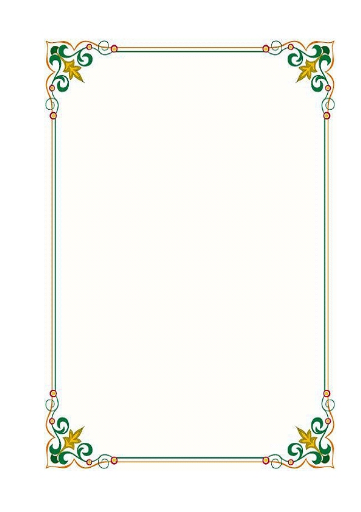
\includegraphics[width=\paperwidth,height=\paperheight]{Figures/bgg4.png}} ;
\end{tikzpicture}
\vskip15mm
\begin{center}
	\resizebox{6cm}{1.1cm}{\calligra Dedication} 
\end{center}
\vfill 
\begin{center}
	\parbox{.85\linewidth}{\centering 
		\baselineskip=8mm 
		\fontfamily{pzc}\selectfont 
		\Large 
This work is dedicated with deep love and gratitude to:
\\[5mm]
My dear parents,
whose unwavering support, sacrifices, and constant prayers have been the foundation of everything I’ve achieved. Your belief in me gave me the strength to persevere through every challenge.
\\[5mm]
My supervisor, Mr. [Mr Salem Mohamed],
whose patient guidance, insightful feedback, and continuous encouragement made this journey not only possible but meaningful. Your dedication, expertise, and belief in my potential have left a lasting impact on me both academically and personally.
\\[5mm]
My beloved sister,
for being my greatest cheerleader and my constant source of emotional support. Your encouragement and care during the toughest moments meant the world to me.
\\[5mm]
My wonderful friend [nial hadjer],
for always being there with kind words, late-night conversations, and unshakable support.
\\[19mm]
}
\end{center}
\vfill 
\thispagestyle{empty}% Dedication page
	%%%%%%%%%%%%%%%%%%%%%%%%%%%% Abstracts in Arabic, English and French %%%%%
	%The abstract pdf file is obtained by compiling separately the abstract.tex file, due to the conflict between the Arabic language in the abstract and the hyperref package
	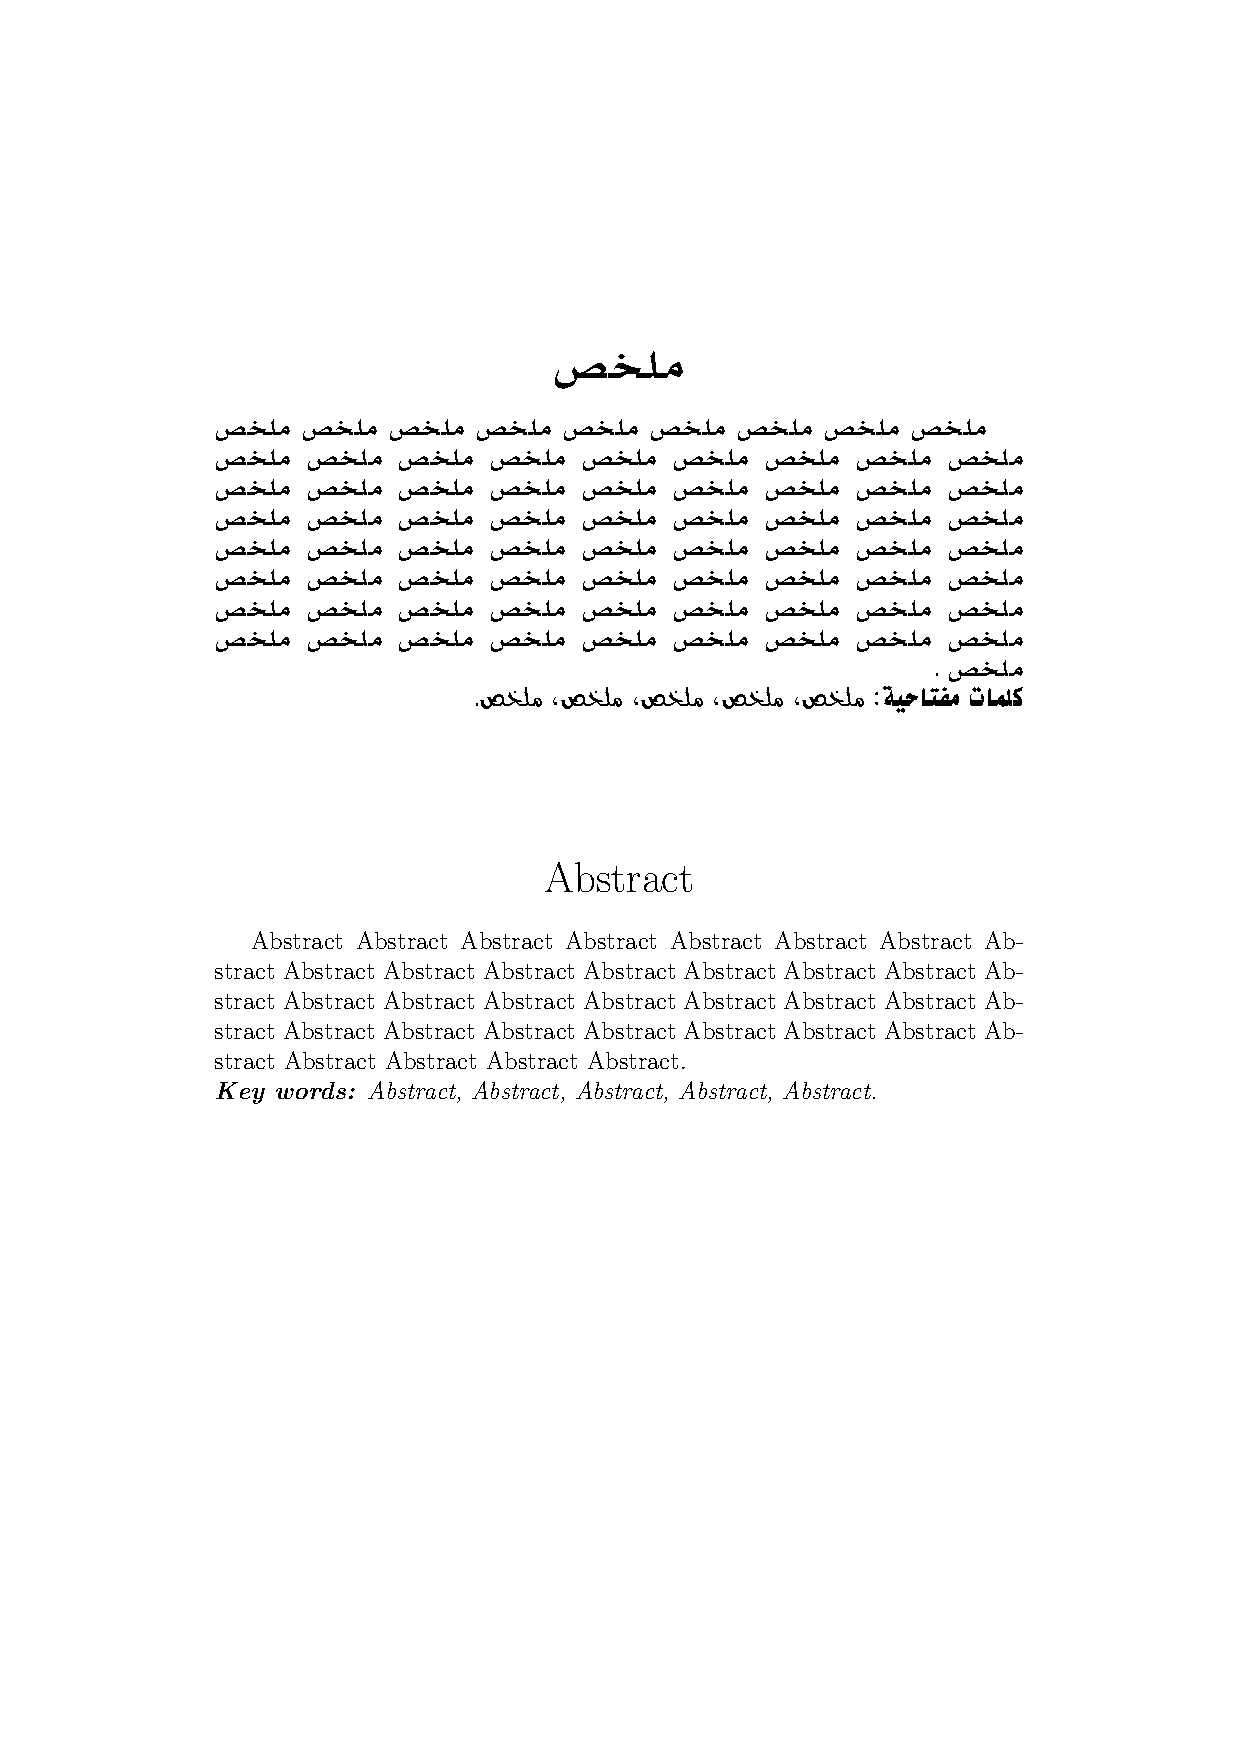
\includepdf[pages=-]{Abstract.pdf}
	%%%%%%%%%%%%%%%%%%%%%%%%%%%% Copyright declaration %%%%%%%%%%%%%%%%%%%%%%%
	% Images sources for copyright purposes 
	%%%\begin{landscape}
	\thispagestyle{empty}
	\begin{center}
		\Huge{\textbf{Sources of Images}} \\
		\normalsize{\textit{for Copyright purposes}}
	\end{center}
	Figure 2.1 from \url{www.site1.com} \\
	Figure 2.3 from \url{www.site2.fr} \\
	Figure 2.5 from \url{www.site3.com} \\
	Figure 2.9 from \url{www.site4.com} \\
	Figure 3.5 from \url{www.site5.com} \\
	Figure 2.3 from \url{www.site2.fr} \\
	Figure 2.5 from \url{www.site3.com} \\
	Figure 2.9 from \url{www.site4.com} \\
	Figure 3.5 from \url{www.site5.com} \\
\end{landscape}

	%\includepdf{Copyright.pdf}
	%%%%%%%%%%%%%%%%%%%%%%%%%%%% Table of contents %%%%%%%%%%%%%%%%%%%%%%%%%%
	\newpage
	\thispagestyle{fancy}
	\fancyhf{}
	\pagestyle{fancy}\lhead{\textbf \footnotesize\it{Contents}} 
	\pagestyle{fancy}\chead{} 
	\pagestyle{fancy}\rhead{}
	\pagestyle{fancy}\lfoot{\textbf {\small\it{Univ-Mascara/Computer Science: 2024}}} 
	\pagestyle{fancy}\cfoot{} 
	\pagestyle{fancy}\rfoot{}
	\pagenumbering{gobble}
	\tableofcontents 
	\setcounter{secnumdepth}{3}
	\setcounter{tocdepth}{3}
	
	%%%%%%%%%%%%%%%%%%%%%%%%%%% List of Figures %%%%%%%%%%%%%%%%%%%%%%%%%%%%
	%%\addcontentsline{toc}{chapter}{List of figures}
	\newpage
	\thispagestyle{fancy}
	\fancyhf{}
	\pagestyle{fancy}\lhead{\textbf \footnotesize\it{List of Figures}} 
	\pagestyle{fancy}\chead{} 
	\pagestyle{fancy}\rhead{}
	\pagestyle{fancy}\lfoot{\textbf {\small\it{Univ-Mascara/Computer Science: 2025}}} 
	\pagestyle{fancy}\cfoot{} 
	\pagestyle{fancy}\rfoot{}
	\pagenumbering{gobble}
	\listoffigures 
	%%%%%%%%%%%%%%%%%%%%%%%%%% List of Tables %%%%%%%%%%%%%%%%%%%%%%%%%%
	%%\addcontentsline{toc}{chapter}{List of tables}
	\newpage
	\thispagestyle{fancy}
	\fancyhf{}
	\pagestyle{fancy}\lhead{\textbf \footnotesize\it{List of Tables}} 
	\pagestyle{fancy}\chead{} 
	\pagestyle{fancy}\rhead{}
	\pagestyle{fancy}\lfoot{\textbf {\small\it{Univ-Mascara/Computer Science: 2025}}} 
	\pagestyle{fancy}\cfoot{} 
	\pagestyle{fancy}\rfoot{}
	\pagenumbering{gobble}
	\listoftables 
	%%%%%%%%%%%%%%%%%%%%%% List of Abbreviations %%%%%%%%%%%%%%%%%%%%%%
	%%\addcontentsline{toc}{chapter}{List of Abbreviations}
	\newpage
	\thispagestyle{fancy}
	\fancyhf{}
	\pagestyle{fancy}\lhead{\textbf \footnotesize\it{List of Abbreviations}} 
	\pagestyle{fancy}\chead{} 
	\pagestyle{fancy}\rhead{}
	\pagestyle{fancy}\lfoot{\textbf {\small\it{Univ-Mascara/Computer Science: 2025}}} 
	\pagestyle{fancy}\cfoot{} 
	\pagestyle{fancy}\rfoot{}
	\pagenumbering{gobble} % To suppress numbering 
	\chapter*{List of Abbreviations }
\pagestyle{fancy}\lhead{\textbf \footnotesize\it{List of Abbreviations}}
\pagestyle{fancy}\lfoot{\textbf {\small\it{Univ-Mascara/Computer Science: 2024}}}
\pagestyle{fancy}\rhead{\textbf \footnotesize\it{}}
\addcontentsline{toc}{chapter}{List of Abbreviations }
%%%%%%%%%%%%%%%%%%%%%%%%%%%%%%%%%%%%%%%%%%%%%%%%%

\begin{tabular}{ll}
	\textbf{BART}:& Bidirectional Auto-Regressive Transformers\\
	\textbf{BERT}:& Bidirectional Encoder Representations from Transformers\\
	\textbf{BLEU}:& Bilingual Evaluation Understudy\\
	\textbf{BRNN}:& Bidirectional Recurrent Neural Network\\
	\textbf{BT}:& Back Translation\\
	\textbf{FFN}:& Feed-Forward Network\\
	\textbf{GPT}:& Generative Pre-trained Transformer\\
	\textbf{GRU}:& Gated Recurrent Units\\
	\textbf{LLM}:& Large Language Model\\
	\textbf{LSTM}:& Long Short-Term Memory\\
	\textbf{MT}:& Machine Translation\\
	\textbf{NLG}:& Natural Language Generation\\
	\textbf{NLP}:& Natural Language Processing\\
	\textbf{NLU}:& Natural Language Understanding\\
	\textbf{NMT}:& Neural Machine Translation\\
	\textbf{RBMT}:& Rule-Based Machine Translation\\
	\textbf{RNN}:& Recurrent Neural Network\\
	\textbf{Seq2Seq}:& Sequence to Sequence\\
	\textbf{SMT}:& Statistical Machine Translation\\
	\textbf{T5}:& Text-to-Text Transfer Transformer\\
\end{tabular} 
	%%%%%%%%%%%%%%%%%%%%% Main document %%%%%%%%%%%%%%%%%%
	\newpage
	\pagenumbering{arabic} 
	\chapter{Introduction}
\pagestyle{fancy}\lhead{\textbf \footnotesize\it{Introduction}}
\pagestyle{fancy}\chead{} \pagestyle{fancy}\rhead{}
\pagestyle{fancy}\lfoot{\textbf {\small\it{Univ-MascaraComputer Science: 2024}}}
\pagestyle{fancy}\cfoot{} \pagestyle{fancy}\rfoot{\thepage}
\pagenumbering{arabic}
%\addcontentsline{toc}{chapter}{General introduction}
%%%%%%%%%%%%%%%%%%%%%%%%%%%%%%%%%%%%
Here goes the Introduction.\\
%%%\newpage
\section{Problem Identification and Motivation}\label{start1}
Context and Motivation
\section{Objectives and Scope}
Create Arabic MT
no DS

\section{Contributions}
Create Corpus
Create Seq2Seq
Use ChatGPT
Survey Arabic Corpora
Survey Arabic MT
\section{Outline of the Thesis}
	\chapter*{PART I:\\BACKGROUND AND RELATED WORK}
\addcontentsline{toc}{chapter}{PART I: BACKGROUND AND RELATED WORK}
	\chapter{Large Language Models (LLMs)}
\pagestyle{fancy}\lhead{\textbf \footnotesize\it{Enhancing Legal Information Access with Retrieval Augmented LLMs for Juridical Data}}
\pagestyle{fancy}\chead{} \pagestyle{fancy}\rhead{}
\pagestyle{fancy}\lfoot{\textbf {\small\it{Univ-Mascara/Computer Science: 2025}}} 
\pagestyle{fancy}\cfoot{} \pagestyle{fancy}\rfoot{\thepage}
%%%%%%%%%%%%%%%%%%%%%%%%%%%%%%%%%%%%%%%%
\section{Introduction} \label{start1}
Large Language Models (LLMs) represent a transformative leap in Natural Language Processing (NLP), allowing machines to perform complex language tasks with remarkable accuracy. From generating coherent text to answering nuanced questions, LLMs have pushed the boundaries of what AI can achieve. This chapter delves into the architecture and principles behind LLMs, their development through scaling and training techniques, and the models that have defined this field. It also addresses the challenges these models face and their expanding role in various real-world applications. 

\section{Natural language processing (NLP)}
Natural Language Processing (NLP) is a field within artificial intelligence (AI) that concentrates on the interaction between computers and human language. It involves the development of algorithms and models  that allow machines to comprehend, interpret, and generate human language in a meaningful context.NLP is crucial for enabling computers to process and respond to human language effectively, as demonstrated by features like Google's predictive text in keyboards and language translation systems that manage multiple languages efficiently \cite{murugan2024nlp}

\subsection{Historical development of (NLP)}
The figure below presents a timeline outlining the key developments in Natural Language Processing (NLP)  beginning with rule-based approaches in the 1950s and progressing through the rise of statistical methods and early neural networks in the late 1980s. It then highlights the impact of deep learning from the 2000s onward, leading to the development of pre-trained models like BERT and GPT. The timeline concludes with the emergence of large language models (LLMs) from 2019 to the present, marking a significant shift in NLP research and applications.
\begin{figure}[htbp]
	\centerline{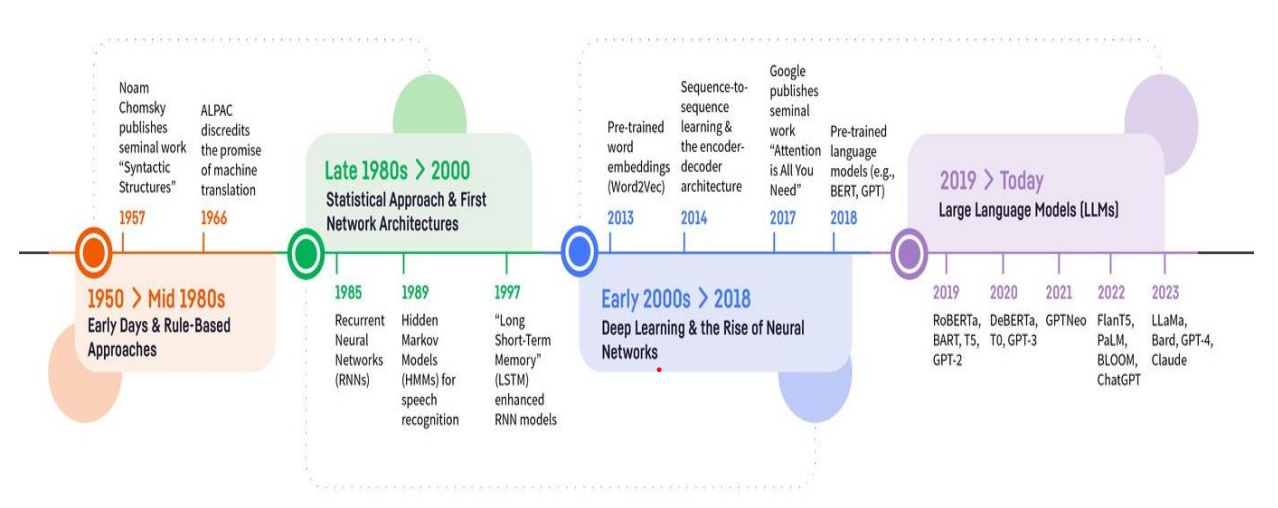
\includegraphics[scale=.7]{Figures/the_historyOf_nlp.png}}
	\caption{The Vauquois triangle, illustrating the foundations of machine translation.}
	\label{the_historyOf_nlp.png}
\end{figure}

\subsection{Importance of natural language processing}

\begin{enumerate}
	\item \textbf{Efficient Data Processing:} NLP enables businesses to process and analyze large volumes of unstructured, text-heavy data that would be challenging to handle otherwise..

	\item \textbf{Understanding Human Language:}NLP can interpret complex language elements, such as acronyms, abbreviations, and context, improving the accuracy of machine learning models..
	
	\item \textbf{Advancements in Technology:}Improvements in deep learning and machine learning have made NLP more effective, expanding the types of data that can be analyzed.
	
	\item \textbf{Natural Interactions:} NLP allows users to interact naturally with AI chatbots and voice assistants, like Siri, without needing to use specific,predefined\cite{techtarget_nlp}.
	
\end{enumerate}

\section{Neural Networks in NLP}
A neural network, or artificial neural network, is a machine learning algorithm inspired by the human brain. It is a key component of deep learning, a branch of machine learning effective in solving complex problems like image recognition and language processing. Unlike traditional computer programs that use a step-by-step algorithmic approach, neural networks learn from examples, mimicking the way neurons in the human brain operate. They consist of interconnected nodes (processing elements) that work together in parallel to solve specific problems. \\
A neural network has three basic sections, or parts, each composed of "nodes." \\ The input layer is the first part, receiving raw data, with each node (or neuron) representing a feature of this data. The hidden layers, which form the intermediate section, perform various transformations and computations, enabling the network to learn complex patterns and relationships. Finally, the output layer, which is the last part, produces the network's output, with the number of nodes corresponding to the desired output classes or regression values \cite{murugan2024nlp}.
\begin{figure}[htbp]
	
	\centerline{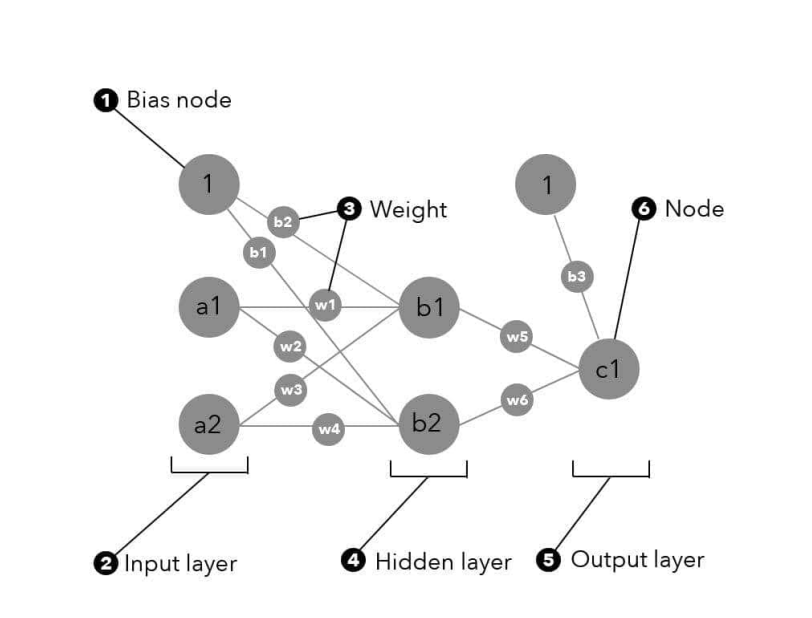
\includegraphics[width=.7\linewidth]{Figures/ANN.png}}
	\caption{Artificial Neural Network (ANN).}
	\label{ANN.png}
\end{figure}  

\subsection{Basics Concepts in Neural Networks}
\textbf{Weights} 


Variables on the edges between nodes that are multiplied with node outputs to form the input for the next layer.Weights are crucial for training and tuning a neural network and are often initialized within a range of -1 to 1.  \\
\textbf{Biases} 


Additional nodes in hidden and output layers that connect to every node within their respective layers but not to the previous layer. Biases add a constant value (typically 1 or -1) to the input of a layer, helping shift the activation function and aiding in effective learning. 
\textbf{Activation Functions} 


These functions introduce non-linearity to the network, enabling it to learn and model complex data patterns. Common activation functions include the sigmoid, hyperbolic tangent (tanh), and rectified linear unit (ReLU). \cite{taylor2017neural}.

\subsection{ Recurrent Neural Networks (RNNs)}
Recurrent Neural Networks (RNNs) are a type of neural networks specifically designed for modeling and processing sequential data, such as text or time series. They are particularly well-suited for handling inputs of variable length by maintaining a dynamic internal state. An RNN comprises a hidden state $h$ and an optional output $y$, and operates over an input sequence $x = (x_1, x_2, \dots, x_t)$.

At each time step $t$, the hidden state $h^{(t)}$ is updated based on the previous hidden state $h^{(t-1)}$ and the current input $x_t$ using a non-linear transition function $f$, as shown in Equation~\ref{eq:rnn_update}:

\begin{equation}
	h^{(t)} = f(h^{(t-1)}, x_t)
	\label{eq:rnn_update}
\end{equation}

The function $f$ can be a simple non-linear activation such as the logistic sigmoid or hyperbolic tangent, or a more complex function such as a Long Short-Term Memory (LSTM) unit or a Gated Recurrent Unit (GRU).
\begin{figure}[htbp]
	
	\centerline{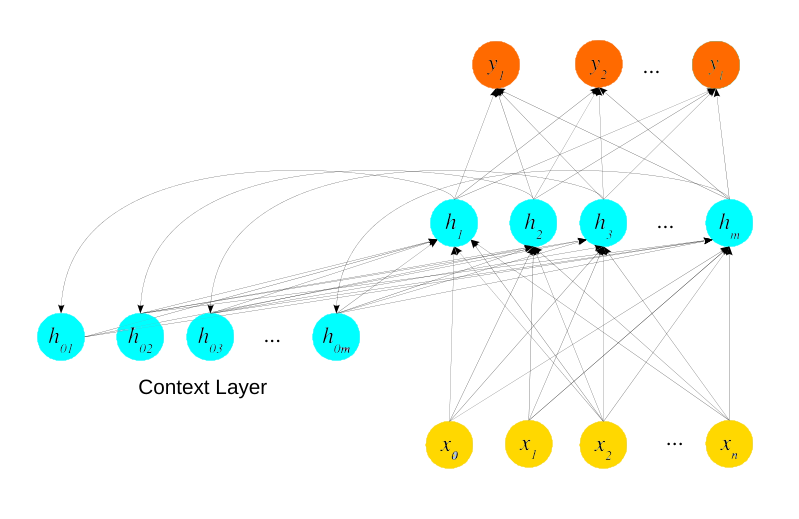
\includegraphics[width=1\linewidth]{Figures/RNN.png}}
	\caption{RNN Architecture.}
	\label{RNN.png}
\end{figure}


This architecture enables RNNs to retain information from previous time steps, allowing the model to capture temporal dependencies and patterns that span across various positions in the sequence. Furthermore, the use of shared parameters across time steps facilitates generalization over sequences of different lengths and enhances the network's ability to learn long-range dependencies.

Despite known challenges, such as difficulties in capturing long-term dependencies due to issues like vanishing gradients, RNNs remain highly effective for tasks that require sequential reasoning or contextual awareness. As a result, they are widely used in applications ranging from time series forecasting to natural language processing.
\cite{cho2014learning} 

\subsection{ Long-Short Term Memory (LSTM)}
Long Short-Term Memory (LSTM) networks, designed by Hochreiter and Schmidhuber, are an improved version of recurrent neural networks (RNNs) designed to learn long-term dependencies in sequential data, making them suitable for tasks like time series forecasting and language translation
They address the limitations of traditional RNNs by introducing a memory cell that maintains information over extended periods. This memory cell is regulated by three gates—input, forget, and output gates—which control the flow of information in and out of the cell as shown in the fig \cite{geeksforgeeks_lstm}
\begin{figure}[htbp]
	\centering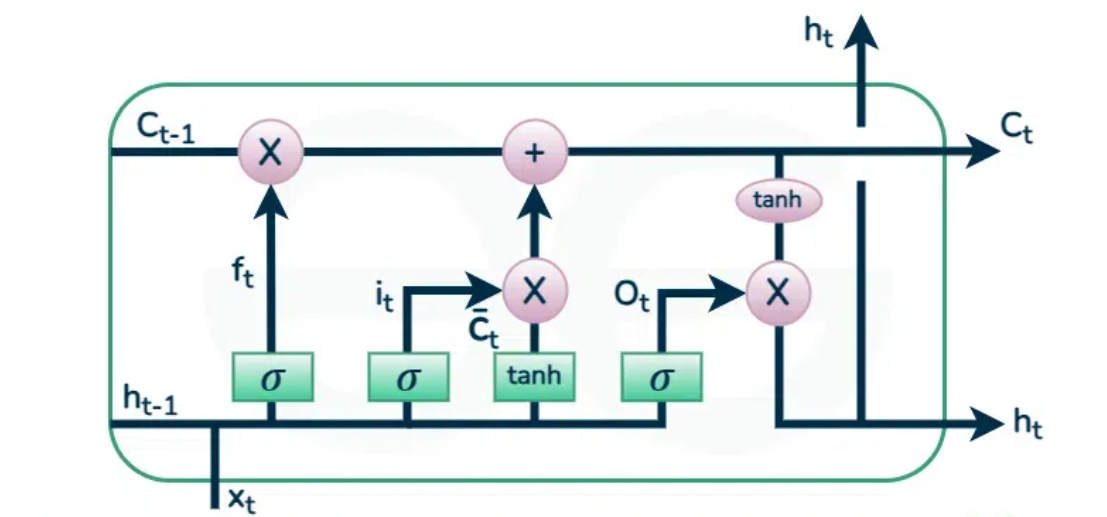
\includegraphics[width=0.9\linewidth]{Figures/LSTM.png}
	\caption{LSTM Architecture.}
	\label{/LSTM.png}
\end{figure}


Forget Gate: Decides what information to discard from the cell state
% Forget Gate
\begin{equation}
	f_t = \sigma \left( W_f \cdot [h_{t-1}, x_t] + b_f \right)
\end{equation}

% Input Gate: Determines what new information to add to the cell state
\begin{equation}
	i_t = \sigma \left( W_i \cdot [h_{t-1}, x_t] + b_i \right)
\end{equation}
\begin{equation}
	\tilde{C}_t = \tanh \left( W_c \cdot [h_{t-1}, x_t] + b_c \right)
\end{equation}

% Cell state update (commonly used but missing in your snippet)
\begin{equation}
	C_t = f_t \odot C_{t-1} + i_t \odot \tilde{C}_t
\end{equation}

% Output Gate: Controls what information to output from the cell state
\begin{equation}
	o_t = \sigma \left( W_o \cdot [h_{t-1}, x_t] + b_o \right)
\end{equation}
\begin{equation}
	h_t = o_t \odot \tanh(C_t)
\end{equation}


It is worth mentioning that Bidirectional LSTM networks extend the traditional LSTM architecture by processing data in both forward and backward directions. This approach enables the network to capture dependencies from both past and future contexts, improving its ability to resolve temporal dependencies. 

Bidirectional LSTMs are particularly effective at handling multidimensional problems, encapsulating spatially and temporally distributed information, and dealing with incomplete data through flexible connection mechanisms \cite{hochreiter1997long}. 
\section{ Transformer Architecture}
The Transformer architecture is a deep learning model introduced in June 2017 by Vaswani et al. from Google Brain. Their paper, titled "Attention Is All You Need," presented a groundbreaking approach to processing sequential data through the use of a self-attention mechanism. This innovative method allows the model to assign different levels of importance to various parts of the input, enabling it to capture long-range dependencies much more effectively than earlier models like RNNs and LSTMs.The original Transformer model is structured as a stack of six layers, where the output of each layer i serves as the input to the subsequent layer i+1, continuing this process until the final prediction is reached.It features a six-layer encoder on the left and a corresponding six-layer decoder on the right,  both of which work together to transform input sequences into meaningful outputs. Each encoder and decoder consists of six identical layers that allow the model to process and generate language efficiently \cite{rothman2021transformers}.
\begin{figure}[htbp]
	
	\centerline{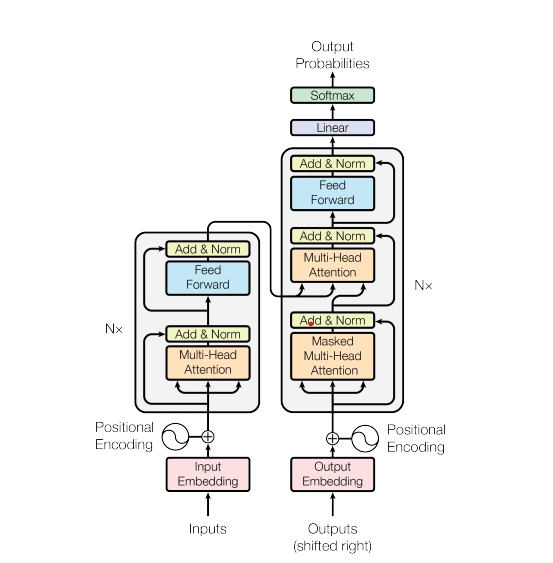
\includegraphics[width=.6\linewidth]{
			Figures/trasformers.png}}
	\caption{The Transformer - model architecture..}
	\label{trasformers.png}
	
\end{figure}
\subsection{Encoder and Decoder Stacks}
\textbf{Encoder}\\ Each layer in the encoder consists of two sub-layers: \\
Multi-head self-attention mechanism: This allows the model to focus on different parts of the input sequence. \\
Position-wise feed-forward network: A fully connected network applied to each position separately and identically. \\
Residual Connections: Residual connections are applied around each sub-layer, followed by layer normalization. The output of each sub-layer is computed as Layer Norm(x + Sublayer(x)). \\
Output Dimension: All sub-layers and embedding layers output vectors of dimension d-model = 512.\\
\textbf{Decoder}\\ Similar to the encoder, the decoder also has 6 identical layers, each containing the same two sub-layers:
Multi-head self-attention mechanism ,
Position-wise feed-forward network. \\
Additional Sub-layer: The decoder includes a third sub-layer that performs multi-head attention over the output of the encoder stack. \\
Residual Connections and Normalization: Like the encoder, residual connections are applied around each sub-layer, followed by layer normalization. \\
Masked Self-Attention: The self-attention mechanism in the decoder is modified to prevent positions from attending to subsequent positions, ensuring that predictions for position i depend only on the known outputs at positions before i \cite{vaswani2017attention}.
\begin{figure}[htbp]
	
	\centerline{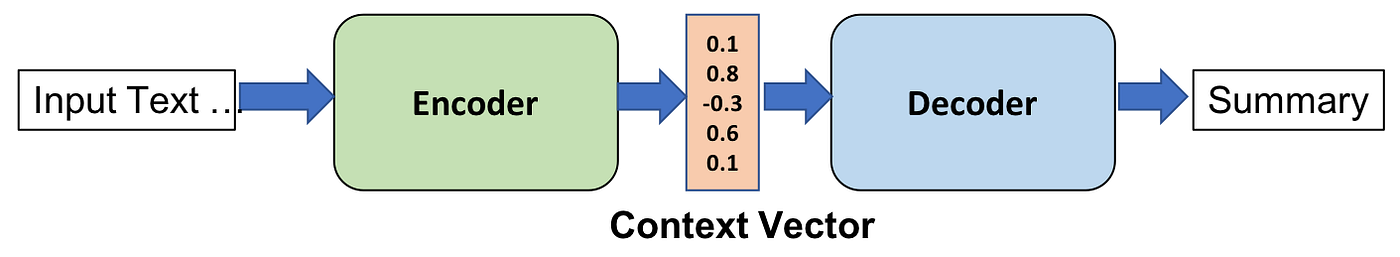
\includegraphics[width=.8\linewidth]{
			Figures/incoderDecoder.png}}
	\caption{Encoder and Decoder Stacks}
	\label{incoderDecoder.png}
	
\end{figure}
\subsection{Self-Attention Mechanism in Transformers}

Self-attention is a fundamental component of the Transformer architecture, enabling the model to dynamically assess the relevance of each token in a sequence relative to others. This mechanism facilitates the capture of contextual dependencies and semantic relationships among words.

The self-attention operation involves three key components derived from the input embeddings: the \textit{Query} ($Q$), \textit{Key} ($K$), and \textit{Value} ($V$) matrices. The attention scores are computed by taking the dot product between the query vector of a token and the key vectors of all tokens in the sequence:

\begin{equation}
	\text{Attention}(Q, K, V) = \text{softmax}\left(\frac{QK^\top}{\sqrt{d_k}}\right)V
\end{equation}

Here, $d_k$ denotes the dimension of the key vectors, which is used to scale the dot product to prevent excessively large values that could hinder gradient flow. The softmax function transforms the scaled scores into a probability distribution, which serves as the attention weights. These weights are then applied to the value vectors to compute a weighted sum, yielding the output representation for each token.

This mechanism allows each token to selectively focus on other relevant tokens, thereby enhancing the model’s capacity to understand complex linguistic patterns~\cite{vaswani2017attention}.
\subsection{Positional Encoding:}
Since self-attention mechanisms do not inherently capture the order of words, positional encoding is added to the word embeddings to provide information about the relative position of each word in the sequence.
These encodings are added directly to the input embeddings, allowing the model to consider both the position and the content of 
each word during processing\cite{alammar2018illustratedtransformer}.
\subsection{Role of Multi-Head Attention}
Multi-head attention is a key enhancement of the self-attention mechanism that significantly improves the model’s representational capacity. Instead of relying on a single attention operation, the mechanism projects the input into multiple distinct sets of Query, Key, and Value vectors, referred to as attention heads. Each head independently performs self-attention, allowing the model to capture diverse contextual relationships from different subspaces of the input representation.

The outputs of all attention heads are then concatenated and linearly transformed, producing a unified representation that integrates the complementary information gathered by each head. This mechanism enhances the model’s ability to capture complex patterns across different positions in the sequence, thereby improving overall performance in a variety of natural language understanding tasks\cite{vaswani2017attention}.

\subsection{The Rise of Transformers in Natural Language Processing}
Transformers have revolutionized the field of Natural Language Processing (NLP) by introducing a powerful and efficient way to handle textual data. This advancement has led to the creation of highly effective models like BERT and GPT, with its deep bidirectional context, excels at understanding and improving performance across various NLP tasks. GPT, on the other hand, is renowned for generating coherent and contextually relevant text, significantly advancing applications such as text generation and translation\cite{devlin2019bert}.\\
\textbf{Scalability:} Transformers efficiently handle large datasets and long sequences, overcoming the limitations of RNNs. This scalability allows for training with billions of parameters, enhancing model capabilities.\\
\textbf{Rich Contextual Understanding: }The self-attention mechanism in transformers captures relationships between words across the entire sequence, enabling deep contextual understanding and more accurate language processing.\\
\textbf{Model Efficiency:} Transformers enable parallel processing, which speeds up training and makes them more efficient than sequential models like RNNs. This efficiency supports the rapid development and deployment of advanced language models\cite{vaswani2017attention}.
\section{ Emergence of Large Language Models (LLMs)}

Large Language Models (LLMs) are advanced artificial intelligence systems designed to process and generate human-like text. They are typically based on transformer architectures and are characterized by their enormous scale, with billions of parameters. LLMs are pre-trained on vast amounts of text data in a self-supervised manner, enabling them to develop a broad understanding of language. They are capable of performing a wide range of tasks with minimal task-specific fine-tuning, often achieving significant performance improvements through few-shot or zero-shot learning\cite{brown2020language}.
\subsection{Scaling in Large Language Models (LLMs)}
Scaling is crucial in the evolution of large language models. The history of scaling shows that increasing both model size and dataset size leads to significant improvements in performance across various NLP tasks. For instance, early work by Brants et al. (2007) demonstrated the benefits of using language models trained on vast datasets, such as 2 trillion tokens, which led to significant advancements in machine translation quality. This was followed by efforts like those of Heafield et al. (2013), who scaled traditional models to Web-scale data, and Jozefowicz et al. (2016), who scaled LSTMs to 1 billion parameters, achieving state-of-the-art results on large benchmarks.The advent of transformer-based models marked a significant shift.Models like BERT, GPT-2, and GPT-3, with their enormous parameter counts—up to 175 billion for GPT-3—demonstrated that scaling up not only the model but also the dataset size yields substantial gains in performance. Researchers like Kaplan et al. (2020) and Hoffmann et al. (2022) studied how scaling affects model performance, proposing power laws that show a predictable relationship between model size, dataset size, and performance. These studies emphasized the importance of scaling for the continued progress of LLMs\cite{touvron2023llama}.
\subsection{Pre-training}
Pre-training is a crucial stage in developing Large Language Models (LLMs), where the model learns from extensive unlabeled datasets through a process called self-supervision. This stage allows the model to recognize and internalize a wide range of linguistic patterns, laying the groundwork for fine-tuning on specific tasks.\\
Several pre-training objectives have been implemented to maximize the effectiveness of this learning process, each offering distinct benefits to the model's performance .\\
\textbf{Full Language Modeling:} Used since GPT-2, this approach trains decoder-only models to predict the next token in a sequence based on previous tokens. This autoregressive method enables models like GPT-3 to generate coherent and contextually relevant text.\\
\textbf{Prefix Language Modeling: }Employed in encoder-decoder and non-causal decoder-only models, this technique uses a non-causal (considering both past and future tokens) prefix for predicting subsequent tokens, offering more flexibility and enhancing the model's adaptability across various language tasks.\\
\textbf{Masked Language Modeling: }Popularized by BERT, this method involves masking certain tokens in the input text and training the model to predict them, helping the model understand word context. An extension, span corruption, masks entire text spans for prediction, further improving contextual comprehension\cite{wang2023language}.\\
\textbf{Unified Language Modeling} refers to an approach that integrates multiple training objectives, including causal, non-causal, and masked language modeling. In this framework, masked language modeling differs from traditional bidirectional attention mechanisms by employing unidirectional attention—processing context either from left-to-right or right-to-left, rather than considering both directions simultaneously\cite{dong2019unified}.
\begin{figure}[h]
	\centering
	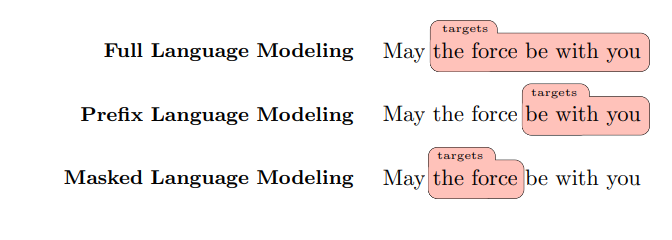
\includegraphics[width=0.6\linewidth]{Figures/pretraining.png}
	\caption{Training Tokenization in Full, Prefix, and Masked Language Modeling.}
\end{figure}
\subsection{Fine-tuning }
Fine-tuning is a key technique for adapting pre-trained large language models (LLMs) to specific downstream tasks. It encompasses several strategies, each serving different objectives. 

One common method is \textbf{transfer learning}, where a pre-trained model is further trained on task-specific data to enhance its performance on targeted applications. This allows models to leverage general language understanding while adapting to more specialized domains.

Another approach is \textbf{instruction tuning}, which involves fine-tuning the model on datasets formatted as instruction-response pairs. These datasets typically include multiple tasks described in natural language, enabling the model to better understand prompts and generalize across various instructions. This method has been particularly effective in improving zero-shot and few-shot performance.

To address ethical and safety concerns, \textbf{alignment tuning} is employed. This involves adjusting the model’s behavior based on human feedback to ensure outputs are helpful, honest, and harmless (the "HHH" criteria). A widely adopted framework for this is reinforcement learning with human feedback (RLHF). RLHF combines reward modeling—where human preferences guide the ranking of responses—with reinforcement learning techniques, such as proximal policy optimization (PPO), to iteratively align model behavior with human values.

These fine-tuning approaches, while powerful, come with trade-offs in terms of data requirements, computational cost, and generalization capabilities. Nonetheless, they remain essential for tailoring LLMs to both functional and ethical requirements across diverse applications.\cite{touvron2023llama}.
\subsection{Few-Shot, One-Shot, and Zero-Shot Learning}
Few-shot, one-shot, and zero-shot learning represent different paradigms of using LLMs without extensive fine-tuning. These methods involve using pre-trained models to perform tasks with minimal task-specific data.\\
\textbf{Few-Shot Learning} involves giving the model a few examples (typically 10-100) of the task during inference. This approach reduces the need for large, task-specific datasets and limits the risk of overfitting to narrow data distributions. However, few-shot results are generally not as strong as those from fully fine-tuned models.\\
\textbf{One-Shot Learning} is similar to few-shot learning but uses only a single example alongside a natural language description of the task. This method mirrors how humans are often instructed for tasks, making it an interesting approach for tasks where providing multiple examples is impractical.\\
\textbf{Zero-Shot Learning} requires the model to perform a task based solely on a natural language description, with no examples provided. While this method offers maximum flexibility and robustness, it is also the most challenging for models. Zero-shot performance is often weaker than few-shot or one-shot, but it represents a significant step towards task-agnostic AI, where models can generalize across a wide range of tasks with minimal human intervention\cite{brown2020language}.
\subsection{Evaluation Datasets and Tasks}
Evaluating Large Language Models (LLMs) is essential for determining their effectiveness and limitations in comprehending and generating human language. This evaluation typically falls into two primary categories:
\begin{itemize}
	\item Natural Language Understanding (NLU):This measures the model's proficiency in comprehending language, encompassing tasks such as sentiment analysis, text classification, natural language inference (NLI), question answering (QA), commonsense reasoning (CR), mathematical reasoning (MR), and reading comprehension (RC).
	\item Natural Language Generation (NLG):This assesses the model's capability to produce text based on given context. It includes tasks like summarization, sentence completion, machine translation (MT), and dialogue generation.
\end{itemize}
\textbf{Benchmarks} play a critical role in evaluating LLMs, providing standardized tests to measure their performance across various tasks:
\begin{itemize}
	\item MMLU: Measures model knowledge from pretraining and evaluates performance in zero-shot and few-shot scenarios across 57 subjects, testing world knowledge and problem-solving abilities.
	\item SuperGLUE: An advanced benchmark that builds on GLUE, assessing tasks like question answering and natural language inference. It is designed to test deeper aspects of language understanding and requires significant advancements in various learning methodologies.
	\item BIG-bench: A large-scale benchmark for evaluating LLMs across diverse tasks including reasoning, creativity, ethics, and domain-specific knowledge.
	\item GLUE: A foundational benchmark for evaluating and analyzing natural language understanding, offering a range of resources for model assessment\cite{Naveed2024}.
\end{itemize}
\section{Popular Models}
Large Language Models (LLMs) like GPT-3, GPT-4, and BERT have revolutionized NLP by leveraging vast datasets such as Common Crawl and WebText. These datasets provide a diverse linguistic foundation, enabling models to perform a wide range of tasks with remarkable accuracy and contextual understanding.
\subsection{GPT-N Models}
GPT models are advanced autoregressive language models that generate substantial and complex machine-produced text from minimal input. They leverage deep learning techniques to mimic human text generation by predicting the current value based on preceding values.
NLP models initially struggled with tasks outside their training sets due to data restrictions. OpenAI addressed this with GPT-1,introduced in 2018.
\begin{itemize}
	\item GPT-1, trained on the BooksCorpus dataset, utilized a 12-layer transformer decoder with self-attention. Its pre-training allowed for zero-shot performance on various tasks, demonstrating the potential of generative language models.
	\item In 2019, GPT-2 improved upon GPT-1 by using a larger dataset and 1.5 billion parameters (compared to GPT-1’s 117 million). It excelled in tasks like translation and summarization, enhancing accuracy in recognizing long-distance relationships.
	\item GPT-3, released later, featured around 175 billion parameters and was trained on the Common Crawl dataset. It could generate human-like text, perform basic math, and write code. Despite its capabilities, its size and cost made it challenging to implement.
	\item GPT-4, launched in March 2023, advanced further with multimodal capabilities and context windows of up to 32,768 tokens. It incorporates reinforcement learning for better alignment with human input and policy\cite{yenduri2023gpt}
\end{itemize}
\subsection{BERT}
BERT (Bidirectional Encoder Representations from Transformers) is a   language representation model that pretrains deep bidirectional representations from unlabeled text by jointly conditioning on both left and right contexts at every layer. This bidirectional strategy allows BERT to be fine-tuned for diverse downstream tasks, such as question answering and natural language inference, by simply appending a single output layer, thereby eliminating the need for extensive architectural modifications.

BERT has demonstrated exceptional performance, establishing new state-of-the-art results across eleven natural language processing benchmarks. Notably, it achieved a GLUE score of 80.5\%, a MultiNLI accuracy of 86.7\%, a SQuAD v1.1 F1 score of 93.2\%, and a SQuAD v2.0 F1 score of 83.1\%. The model's elegant design, coupled with its empirical success, underscores its versatility and efficacy as a powerful tool for a wide array of natural language processing applications.
\cite{devlin2019bert}.
\subsection{T5}
The T5 (Text-To-Text Transfer Transformer) model represents a unified framework for natural language processing (NLP), designed to address various text processing tasks by treating them as "text-to-text" problems. This approach involves converting all tasks into a format where both input and output are text, allowing the same model, objective, and training procedure to be applied across different tasks. T5 leverages extensive pre-training on a large, unlabeled dataset, enabling it to develop general-purpose knowledge that enhances its performance on a range of NLP tasks, such as question answering, document summarization, and sentiment classification\cite{raffel2023exploring}.
\subsection{LLAMA2}
Llama 2 introduces a new family of transformer-based language models available in both foundation and fine-tuned chat variants. These models incorporate architectural enhancements through optimized training procedures, refined pretraining datasets, and advanced fine-tuning techniques including reinforcement learning from human feedback. Empirical evaluations reveal that Llama 2 outperforms its predecessors and other competitive benchmarks across a range of natural language processing tasks, demonstrating notable improvements in accuracy, safety, and generalization. Its open release not only promotes transparency and reproducibility but also fosters collaborative advancements in the field\cite{touvron2023llama2openfoundation}.

\subsection{Jais}
Jais and Jais-chat are advanced Arabic-centric large language models built on a GPT-3 decoder-only architecture. Pretrained on a diverse dataset of Arabic and English texts including programming language source code—these 13-billion-parameter models excel in Arabic knowledge and reasoning, outperforming existing open Arabic and multilingual models. Notably, they also remain competitive in English tasks despite limited English data. We detail their training, fine-tuning, safety alignment, and evaluation, and release both the foundational Jais and the instruction-tuned Jais-chat variants to foster further research on Arabic LLMs\cite{sengupta2023jaisjaischatarabiccentricfoundation}.

\section{Limitations of Large Language Models}
LLMs have greatly advanced NLP, but they also present challenges As these models scale, they encounter new challenges in scalability, privacy, and real-time processing. Several studies have examined the inherent limitations of large language models (LLMs). Notably, \cite{Bender2021} and \cite{Naveed2024} highlight critical challenges that affect the performance and reliability of these models applications.
\subsection{ Computational Cost}
Training large language models (LLMs) demands significant computational resources, leading to higher production costs and environmental concerns due to the substantial energy used in large-scale training. Although enhancing computational resources can boost performance, the gains diminish over time when the size of the model and dataset stay constant, adhering to the power law of diminishing returns.
\subsection{Bias and Ethical Concerns}
The training data for LLMs often encapsulates various social, cultural, and linguistic biases, which the models can inadvertently learn and propagate. This bias can manifest in outputs that reinforce stereotypes or display partiality, raising significant ethical concerns. Addressing these issues is crucial for ensuring fairness and mitigating unintended consequences in real-world applications.
\subsection{ Hallucinations}
LLMs sometimes produce "hallucinations," or responses that, despite appearing plausible, are incorrect or do not match the provided information. These hallucinations can be classified into three types:

\begin{itemize}
	\item Input-conflicting hallucination: When the model generates responses that do not align with the user's input.
	\item Context-conflicting hallucination: When the model produces content that contradicts information it has previously generated.
	\item Fact-conflicting hallucination: When the model creates responses that conflict with established knowledge.
\end{itemize}
\subsection{Overfitting}
Despite their advanced learning abilities, they can overfit to noisy or unusual patterns in their large training datasets, which may result in generating nonsensical responses. The ongoing discussion about Memorization versus Generalization in LLMs revolves around finding an optimal balance. Memorization helps the model retain specific details from its training, allowing it to answer precise questions accurately. On the other hand, generalization enables the model to make predictions and generate responses for new, unseen inputs, which is crucial for handling diverse real-world tasks. The challenge is to find the right balance: excessive memorization can lead to overfitting, reducing the model's flexibility and ability to handle novel inputs.

\section{Domains of Application}
The use of Large Language Models (LLMs) in various downstream tasks has become increasingly prevalent in both AI research and industry, with new applications being identified and explored regularly. These models, which excel at understanding and generating human-like text, are finding valuable applications across diverse fields. 
\subsection{Legal Information and Law}
Large language models (LLMs) are increasingly influential in the legal sector, enhancing the analysis and processing of extensive legal texts. Their ability to manage and interpret large datasets supports tasks such as document classification, information retrieval, and even judicial outcome prediction. For instance, \cite{Chalk2020} presents Legal-BERT, adapts the BERT architecture specifically for legal applications, yielding notable improvements in handling legal documents. Similarly, \cite{Bommarito2018} investigated the use of LLMs in forecasting Supreme Court decisions, demonstrating their potential to contribute to legal analytics and reasoning. These advancements underscore the transformative impact of LLMs on legal research, offering new tools to improve the efficiency and accuracy of legal practice.

\subsection{Cybersecurity}
large Language Models (LLMs) have garnered significant attention in the field of cybersecurity. Recent research has highlighted their potential in addressing software bugs created by human developers and identifying cybersecurity threats. For example, Arora et al. have proposed methods for utilizing LLMs to evaluate cyber threats on social media through sentiment analysis. LLMs are also employed to detect cybersecurity-related information in Open Source Intelligence (OSINT), aiding in the identification of potential cyber threats. Additionally, LLMs have shown promise in detecting scams, such as phishing. Initial tests with models like GPT-3.5 and GPT-4 have demonstrated their ability to recognize common phishing indicators in emails. While LLMs exhibit considerable potential in cybersecurity, improving their reasoning abilities could enhance their effectiveness further, such as in uncovering zero-day vulnerabilities in open-source software by analyzing logic and source code\cite{helwe2024}.
\subsection{Medicine}
The integration of Large Language Models (LLMs) into medicine is transforming both healthcare delivery and research. In clinical settings, LLMs are increasingly utilized in decision support systems to offer evidence-based treatment recommendations. By analyzing patient data and medical literature, these models can assist in diagnosing conditions, suggesting relevant tests, and proposing effective treatment options. Additionally, LLMs improve patient interactions through applications like chatbots that answer questions about symptoms and medications, schedule appointments, and provide health advice.\\
In medical research, LLMs help sift through vast amounts of literature to extract, filter, and summarize relevant information, identify key studies, and predict future research directions. They also play a role in medical education by generating training materials, creating exam questions, explaining complex topics, and offering personalized feedback. Furthermore, LLMs simulate patient interactions, aiding students in honing their clinical skills \cite{Naveed2024}.
\subsection{journalism}
Large Language Models (LLMs) offer valuable support to journalists, especially in fact-checking and news verification. They can process and cross-reference large volumes of data with established knowledge bases. Research has demonstrated that LLMs, such as GPT-3.5, can be used to detect fake news by providing rationales that enhance other models like BERT, which can then be fine-tuned for this purpose .
In addition to fact-checking, LLMs are useful for analyzing political debates, helping journalists to identify key themes, monitor how discussions evolve, and evaluate sentiments. They can also assist in detecting logical fallacies and underlying motives in political discourse and propaganda . By enhancing their reasoning capabilities, LLMs can uncover deeper insights into propaganda and misinformation, making them a powerful tool for modern journalism\cite{helwe2024}.
\section{Conclusion}
This chapter has outlined the evolution and significance of Natural Language Processing (NLP), from early neural networks to advanced Large Language Models (LLMs). We covered key concepts in neural networks and the transformative impact of the Transformer architecture. We also discussed various challenges. Finally, the chapter reviewed the applications of LLMs in fields like Legal Information and Law, cybersecurity, medicine, and journalism, showcasing their potential and the ongoing need for further development.

Although LLMs have demonstrated promising applications in the legal sector, their influence is still constrained by practical limitations and contextual challenges. Recognizing these gaps, the next chapter explores Retrieval-Augmented Generation (RAG) as a novel approach to enhance legal information processing. This discussion will particularly focus on how RAG can be applied within the Algerian legal framework to address existing shortcomings and improve accessibility and accuracy in legal data management.

	\chapter{RAG (Retrieval-Augmented Generation)}
\pagestyle{fancy}\lhead{\textbf \footnotesize\it{Enhancing Legal Information Access with Retrieval Augmented LLMs for Juridical Data}}
\pagestyle{fancy}\chead{} \pagestyle{fancy}\rhead{}
\pagestyle{fancy}\lfoot{\textbf {\small\it{Univ-Mascara/Computer Science: 2025}}} 
\pagestyle{fancy}\cfoot{} \pagestyle{fancy}\rfoot{\thepage}
%%%%%%%%%%%%%%%%%%%%%%%%%%%%%%%%%%%%%%%%
\section{ Introduction}\label{start2}

Large language models (LLMs) have seen significant advancements but face challenges, particularly in tasks that demand extensive knowledge or deal with queries beyond their training data. These limitations often result in inaccuracies or “hallucinations.” To address this, Retrieval-Augmented Generation (RAG) supplements LLMs by retrieving relevant document chunks from external knowledge sources based on semantic similarity. By doing so, RAG helps reduce factual errors, allowing LLMs to produce more accurate content. This has led to the widespread adoption of RAG, particularly in chatbots and other real-world applications, making it a crucial technology in advancing the capabilities of LLMs.
\section{Fundamentals of Retrieval-Augmented Generation}
RAG represents a significant advancement in the capabilities of large language models (LLMs) by integrating external knowledge retrieval with the generation of text. Understanding the individual components of retrieval and generation is essential to appreciate how their synergy improves the overall performance of RAG systems.
\subsection{Definition of RAG}
Retrieval-Augmented Generation (RAG) is a technique that leverages the strengths of pre-trained large language models (LLMs) and external data sources. By merging the generative abilities of LLMs like GPT-3 or GPT-4 with the accuracy of specialized data search mechanisms, RAG systems can generate more sophisticated and contextually relevant responses\cite{selvaraj2024}.
\subsection{Historical Development of RAG}
The foundations of Retrieval-Augmented Generation (RAG) can be traced back to traditional information retrieval (IR) systems,  Early models primarily relied on keyword matching and simple ranking mechanisms to retrieve relevant documents from databases, establishing a basic framework for information access. The landscape began to shift with the rise of neural networks in the 2010s. Notable innovations like Word2Vec and Transformer-based architectures enabled retrieval methods to incorporate deeper semantic understanding, paving the way for more sophisticated document retrieval processes.
A significant advancement occurred with the introduction of dense passage retrieval (DPR) in 2020, which utilized bi-encoder architectures to map both queries and documents into dense vector spaces. 
The integration of these advanced retrieval techniques with large language models (LLMs) became a focal point as models like GPT-3 gained prominence. Researchers explored how LLMs could be augmented with retrieval capabilities, leading to the development of RAG systems that leverage the strengths of both retrieval and generative capabilities\cite{gao2024retrieval}.
\subsection{ Differences Between RAG and Fine-Tuning}
The enhancement of large language models (LLMs) has gained significant interest due to their increasing use. Among the various optimization strategies for LLMs, Retrieval-Augmented Generation (RAG) is often compared to fine-tuning (FT) and prompt engineering. Each method possesses unique attributes,
\begin{enumerate}
	\item Methodological Characteristics :\\
	RAG is compared to providing a tailored textbook for information retrieval, making it suitable for precise information retrieval tasks. It excels in dynamic environments with real-time knowledge updates. \\
	Fine-tuning is likened to a student internalizing knowledge, making it more static and suitable for replicating specific structures, styles, or formats.
	\item External Knowledge and Adaptation: \\
	RAG relies on external knowledge sources and allows for high interpretability but may involve higher latency and ethical considerations regarding data retrieval. \\
	Fine-tuning requires retraining for updates and involves significant computational resources for dataset preparation and training. It enables deep customization of the model’s behavior but may struggle with unfamiliar data.
	\item Performance: \\ RAG consistently outperforms unsupervised fine-tuning in knowledge-intensive tasks, particularly for both previously encountered and new knowledge.
	LLMs often struggle to learn new factual information through unsupervised fine-tuning.
	\item Use Cases and Combination: \\
	The choice between RAG and fine-tuning depends on specific needs for data dynamics, customization, and computational capabilities. They are not mutually exclusive; their combined use may yield optimal performance and often requires multiple iterations to refine the results \cite{gao2024retrieval}.
	
\end{enumerate}
\section{Types of RAG Systems}
The RAG research field is continuously evolving, with three main stages: Naive RAG, Advanced RAG, and Modular RAG.
\subsection{Naive RAG}
Naive RAG, a foundational approach in Retrieval-Augmented Generation, operates on a straightforward "Retrieve-Read-Generate" paradigm. This method involves three primary steps:

\begin{itemize}
	\item Indexing: Raw data is cleaned, extracted, and converted into a uniform text format. It's then segmented into smaller chunks and encoded into vector representations using an embedding model. These vectors are stored in a vector database for efficient similarity searches.
	\item Retrieval: When a user query is received, it's encoded into a vector and compared to the indexed chunks. The top K most similar chunks are retrieved and included in the prompt for the language model.
	\item Generation: The query and retrieved chunks are combined into a prompt, which is fed to a large language model. The model generates a response based on the provided context and its internal knowledge.
\end{itemize}
While Naive RAG offers a basic framework, it faces several challenges in 
\begin{itemize}
	\item Retrieval Issues: The retrieval process can be imprecise, leading to the selection of irrelevant or missing information.
	\item Generation Challenges: The language model may hallucinate, generating content not supported by the retrieved context. It may also produce irrelevant, toxic, or biased outputs.
	\item Augmentation Difficulties: Integrating retrieved information into the generation process can be challenging, leading to disjointed or redundant responses.
\end{itemize}
To address these limitations, more sophisticated RAG techniques have emerged, which we will explore in the next section.
\subsection{Advanced RAG}
Taking aim at the shortcomings of Naive RAG, Advanced RAG introduces specific improvements to enhance retrieval quality. This approach utilizes pre-retrieval and post-retrieval strategies.
\subsubsection{Pre-retrieval Strategies:}
\begin{itemize}
	\item Enhanced Indexing: Advanced RAG tackles indexing issues through a sliding window approach, finer segmentation of data, and inclusion of metadata. Additionally, it optimizes the retrieval process by employing various methods.
	\item Query Optimization: This stage focuses on refining the user's initial query to make it clearer and more suitable for retrieval. Techniques like query rewriting, transformation, and expansion are commonly used.
\end{itemize}
\subsubsection{Post-Retrieval Strategies:}
\begin{itemize}
	\item Re-ranking Chunks: After relevant information is retrieved, Advanced RAG prioritizes the most relevant content by re-ranking the retrieved chunks and placing them strategically within the prompt.
	\item Context Compression: To avoid overwhelming the LLM with too much information, post-retrieval efforts focus on selecting the most essential parts of the retrieved context, highlighting critical sections, and compressing the data to be processed.
\end{itemize}
By addressing indexing issues and refining the query and retrieved information, Advanced RAG aims to improve the overall accuracy and relevance of the generated response.
\subsection{Modular RAG} 
Modular RAG represents the latest evolution in RAG, offering greater adaptability. it introduces specialized modules and innovative patterns to enhance retrieval and processing capabilities.
\subsubsection{New Modules}
\begin{itemize}
	\item Search Module: Adapts to specific scenarios by leveraging LLM-generated code and query languages to search across various data sources.
	\item RAG Fusion: Employs a multi-query strategy to expand user queries, uncover both explicit and implicit knowledge, and improve retrieval results.
	\item Memory Module: Leverages the LLM's memory to guide retrieval and create an unbounded memory pool, aligning the text more closely with data distribution.
	\item Routing Module: Navigates through diverse data sources, selecting the optimal pathway for a query based on its specific needs.
	\item Predict Module: Reduces redundancy and noise by generating relevant context directly through the LLM.
	\item Task Adapter Module: Tailors RAG to various downstream tasks by automating prompt retrieval and creating task-specific retrievers.
\end{itemize}
\subsubsection{New Patterns} 
\begin{itemize}
	\item Flexible Module Arrangement: Modular RAG allows for the substitution and reconfiguration of modules to address specific challenges, surpassing the fixed structures of previous RAG paradigms.
	\item Innovative Retrieval Strategies: Techniques like Rewrite-Retrieve-Read, Generate-Read, and Recite-Read leverage the LLM's capabilities to refine queries, generate content, and retrieve information from model weights.
	\item Hybrid Retrieval: Combines keyword, semantic, and vector searches to cater to diverse queries, improving retrieval relevance.
	\item Dynamic Module Interaction: Frameworks like Demonstrate-Search-Predict and ITERRETGEN demonstrate the dynamic use of module outputs to enhance each other's functionality.
	\item Adaptive Retrieval: Techniques like FLARE and Self-RAG evaluate the necessity of retrieval based on different scenarios, allowing for a more flexible and efficient approach.
	
\end{itemize}
\section{Core Components of RAG}
The core components of Retrieval-Augmented Generation (RAG) systems consist of a retrieval mechanism, a generation process, and augmentation techniques. These elements work together to enhance the model's ability to access relevant external information, generate coherent and contextually appropriate responses, and improve overall performance in knowledge-intensive tasks.
\subsection{ Retrieval Mechanism}
RAG systems combine parametric memory (a pre-trained language model) with non-parametric memory (a retrieval mechanism). The retrieval mechanism allows RAG models to access external information sources (e.g., Wikipedia), and this process is central to improving the model's ability to generate factual and accurate outputs \cite{lewis2020retrieval}.
\begin{itemize}
	\item Traditional Techniques: \\
	Classical retrieval methods include \textbf{TF-IDF and BM25}, which rely on sparse vector representations based on term frequencies. These methods use exact keyword matching, making them limited in semantic understanding.
	\item Modern Retrieval Approaches:\\
	\textbf{ Dense Passage Retrieval (DPR): }This approach utilizes dense vector representations learned by neural models like BERT to encode both the query and document. It allows for a more semantic understanding of the content, making retrieval more effective. DPR, for example, computes the similarity between the query and documents using Maximum Inner Product Search (MIPS), which finds the closest passages based on the dense vector space.
	\item Implementation in RAG:\\ In RAG, dense retrieval methods are often paired with techniques like \textbf{Maximum Inner Product Search} (MIPS), which efficiently matches query and document embeddings. This enables the system to return the most relevant documents for subsequent generation \cite{karpukhin2020dense}.
	
\end{itemize}
\subsection{Generation Process}
The generation in RAG occurs through a combination of retrieved passages and the input query.\\
Large Language Models (LLMs) like BART or T5 are utilized for this generation, leveraging their advanced capabilities in understanding and producing human-like text. The retrieval component supplies external context, which the generator conditions on to formulate a response.This context is crucial, as it enriches the LLM's understanding, enabling it to incorporate real-time, relevant information. Moreover, the generation process benefits from the LLM's ability to synthesize information, allowing it to create responses that are not only coherent but also informed by the latest data, thus improving accuracy and relevance in knowledge-intensive tasks \cite{lewis2020retrieval}. \\
Two models have been proposed in RAG:
\begin{itemize}
	\item \textbf{RAG-Sequence} uses the same document to generate the entire sequence of output. It marginalizes over the top K retrieved documents to produce a final answer.
	\item \textbf{RAG-Token} allows different tokens in the output sequence to be generated based on different documents, making it more flexible when combining information from various
\end{itemize}
\subsection{ Augmentation Techniques}
The augmentation of the retrieval process in Retrieval-Augmented Generation (RAG) systems focuses on improving how queries are refined and how relevant information is retrieved for downstream generation tasks. Key augmentation methods include.
\begin{itemize}
	\item \textbf{Query Augmentation:} In traditional retrieval pipelines, user queries are often under-specified or ambiguous, leading to poor retrieval performance. Query augmentation involves dynamically rewriting the user's query to better match the documents in the knowledge base. This can be done by leveraging large language models (LLMs) to generate tailored queries or synthetic questions and answers (QAs) that better align with the search objective​
	\item \textbf{Synthetic QA Generation:} Instead of using raw document chunks, retrieval is enhanced by generating and embedding synthetic QA pairs from documents. This helps to capture the semantic essence of long texts more effectively, reducing noise and improving retrieval precision. These synthetic QAs can be used to rewrite the user query, making it more specific to the task at hand \cite{mombaerts2024meta}.
\end{itemize}
\begin{figure}
	\centering
	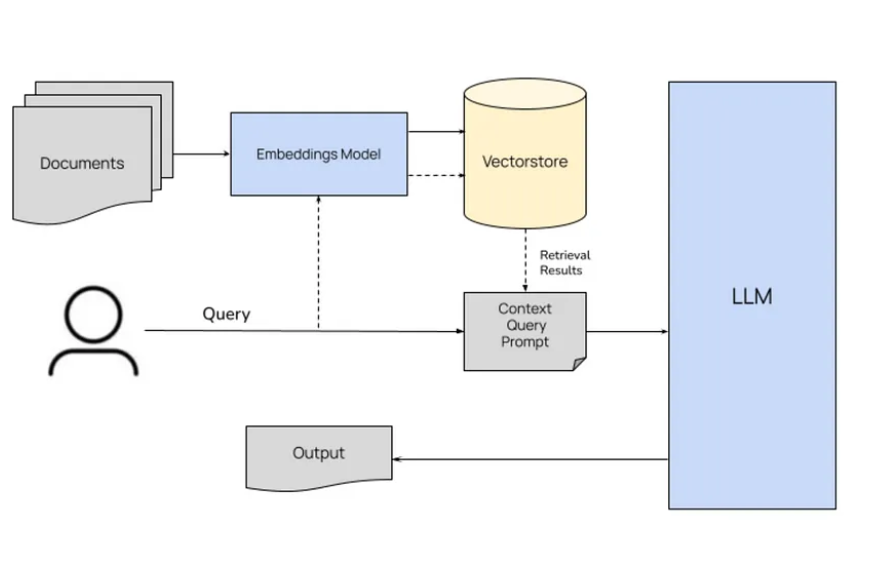
\includegraphics[width=0.9\linewidth]{Figures/rag_architectur.png}
	\caption{Rag architecture}
	\label{rag_architectur.png}
\end{figure}
\section{Training and Fine-Tuning RAG Models}
Training and fine-tuning are essential steps in enhancing the performance of RAG models by optimizing both the retriever and generator components leading to more coherent, relevant, and accurate responses.
\subsection{Training the Retriever}
A powerful technique for improving retrieval relevance involves training the retriever model using \textbf{contrastive learning}. This approach aims to maximize the similarity between query and relevant document embeddings while minimizing the similarity between query and irrelevant document embeddings. By training the model on numerous positive (relevant) and negative (irrelevant) pairs, the retriever learns to effectively distinguish between relevant and irrelevant information\cite{sbert2024}.
\section{Task and Evaluation}
The rapid development and increasing use of Retrieval-Augmented Generation (RAG) models in NLP have made their evaluation a critical area of research within the LLM community. This section covers the primary downstream tasks associated with RAG, the datasets used, and the methods for evaluating RAG systems \cite{zhou2020trustworthiness}.
\subsection{Factuality}
\begin{itemize}
	\item Fact-Checking Benchmarks: Using datasets like FEVER and SQuAD to evaluate the model's ability to identify and correct factual errors.
	\item Adversarial Testing: Creating adversarial examples to test the model's robustness against misleading information.
	\item Contextual Understanding: Assessing the model's ability to understand the context of a query and provide accurate answers.
\end{itemize}
\subsection{ Robustness}
\begin{itemize}
	\item Noise Injection: Introducing noise into the retrieved documents to test the model's ability to handle imperfect information.
	\item Adversarial Attacks: Evaluating the model's resilience to attacks that aim to manipulate its outputs.
	\item Domain Adaptation: Testing the model's ability to adapt to new domains and data distributions.
\end{itemize}
\subsection{Fairness}
\begin{itemize}
	
	\item Bias Detection: Identifying and quantifying biases in the training data and model outputs.
	\item Fairness Metrics: Using metrics like demographic parity and equalized odds to evaluate the model's fairness.
	\item Mitigation Techniques: Implementing techniques like debiasing and fairness constraints to mitigate biases.
\end{itemize}
\subsection{Objective Metrics:}
\begin{itemize}
	\item Accuracy: Precision, recall, and F1-score for evaluating the correctness of the generated responses.
	\item Consistency: Measuring the consistency of the model's outputs across different queries and contexts.
	\item Coherence: Assessing the coherence and fluency of the generated text.
\end{itemize}
\subsection{Subjective Metrics}
\begin{itemize}
	\item Human Evaluation: Using human raters to evaluate the quality of the generated responses.
	\item User Studies: Conducting user studies to gather feedback on the user experience
\end{itemize}
\section{Limitations}
While RAG has gained significant traction across diverse applications, it still faces certain limitations in terms of effectiveness and efficiency\cite{zhao2024retrieval}.
\subsection{Noisy Retrieval Results}
\begin{itemize}
	\item Retrieval Quality: The quality of retrieved information can be affected by factors like indexing techniques, query formulation, and the underlying dataset.
	\item Hallucinations: Noisy or irrelevant information can lead to the generation of hallucinated or factually incorrect responses.
	\item Contextual Understanding: The LLM may struggle to understand the context of the retrieved information, especially if it's poorly formatted or contains inconsistencies.
\end{itemize}
\subsection{Extra Overhead}
\begin{itemize}
	\item Computational Cost: Retrieval and processing additional information can increase computational costs, especially for large-scale models and complex queries.
	\item Latency: Retrieval and processing can introduce latency, impacting the real-time performance of RAG systems.
	\item Complexity: Implementing and deploying RAG systems requires careful consideration of various factors, including data preparation, model selection, and system architecture.
\end{itemize}
\subsection{Interaction of Retrieval and Generation}
\begin{itemize}
	\item Aligning the goals of the retriever and generator is challenging.
	\item Optimizing the interaction between the two components requires careful design and tuning.
	\item The impact of various factors, such as metric selection and hyperparameter tuning, on RAG performance is still not fully understood.
	\item
	
\end{itemize}
\subsection{Long Context Generation:}

\begin{itemize}
	\item Context Length Limits: LLMs have limitations on the amount of context they can process at once.
	\item Information Loss: Long documents may be truncated or summarized, leading to loss of important information.
	\item Computational Cost: Processing long contexts can be computationally expensive.
\end{itemize}
\newpage
\section{Conclusion}
This chapter provided an overview of Retrieval-Augmented Generation (RAG), highlighting its significance in natural language processing. We discussed the key concepts of retrieval and generation, emphasizing the advantages of their combination in enhancing language model capabilities. The historical development of RAG was explored, along with its core components, including the retrieval mechanism, generation process, and augmentation techniques. Additionally, we examined various downstream tasks and evaluation targets, illustrating RAG's versatility in applications like open-domain question answering and fact verification. Overall, RAG represents a promising advancement in knowledge-intensive tasks, paving the way for further research and innovation in the field. 
	\chapter{k Selection in Retrieval}
\section{Introduction}
Retrieval-Augmented Generation (RAG) systems enhance language models by grounding responses in externally retrieved documents.A critical challenge in these systems is determining the optimal number of documents (k) to retrieve for a given query.Current approaches fall into three categories: static k selection, which uses a fixed number of retrieved documents; dynamic k selection, which adjusts k based on query  characteristics; and hybrid approaches, which combine both strategies.In this chapter, we first explore methods, highlighting their strengths and limitations We then introduce our novel hybrid dynamic selection algorithm provide detailed description of its methodology and present experimental results that demonstrate the effectiveness of its performance . 
%\section {The Role of k in Retrieval-Augmented Generation}
%The number of retrieved documents (k) is a critical parameter in Retrieval-Augmented Generation (RAG) that has a direct impact on the retrieval and generation phases. Choosing the right k ensures that the system retrieves enough relevant information. 
\section{Defining k: The Number of Retrieved Documents}
the parameter k denotes the number of documents or passages retrieved from an external knowledge base. This retrieval process is managed by the retriever component\cite{pareto2024rag},which identifies the top k relevant documents based on similarity to the query typically using embedding-based search\cite{Rossi_2024} (e.g., dense retrieval with FAISS, BM25, or hybrid methods) Subsequently, these documents are passed to the generator, typically a language model, which synthesizes the final response by integrating the retrieved 
\begin{figure}[h]
	\centering
	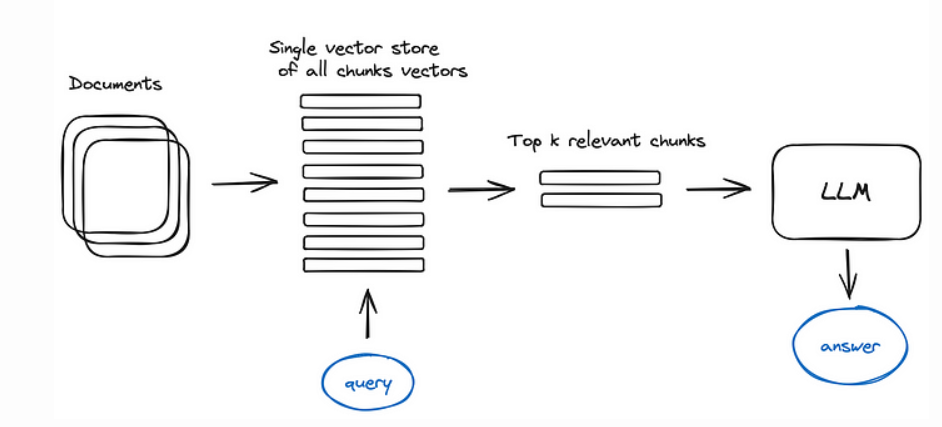
\includegraphics[width=0.9\linewidth]{Figures/topk.png}
	\caption{Basic retrieval}
	\label{rag_retrival.png}
	
\end{figure}
\newline
\section{Impact of k on Retrieval Performance}
The retriever's effectiveness in identifying relevant documents depends on k. Key impacts include :
\subsection{Recall vs. Precision} 
When a user conducts a search query, the outcomes from the database can be grouped into four distinct types based on relevance and retrieval status \cite{geeksforgeeks2022precision}:
\begin{itemize}
	\item {Relevant and Retrieved:} Documents that both address the user’s query and appear in the search results.
	\item {Relevant and Not Retrieved:} Useful documents that answer the query but are not included in the results.
	
	\item {Non-Relevant and Retrieved:} Documents that appear in the results but lack meaningful value for the query.
	 
	\item {Non-Relevant and Not Retrieved:} Irrelevant documents excluded from the results.
\end{itemize}


\textbf{Precision@k}: evaluates the proportion of relevant documents within the top k retrieved results. This metric is particularly valuable in scenarios where the focus is on delivering highly relevant information quickly, rather than ensuring complete coverage such as ,recommendation systems or search engines\cite{deconvoluteai2024metrics}.


\[
\text{Precision@k} = \frac{\text{Number of Relevant Items Retrieved in Top k}}{k}
\]

\textbf{Example}
Suppose we have a dataset of 10 documents. If we retrieve \( k = 4 \) documents and find that 3 of them are relevant to the query:

\begin{itemize}
	\item \textbf{Dataset}: [doc1, doc2, doc3, doc4, doc5, doc6, doc7, doc8, doc9, doc10]
	\item \textbf{Retrieved}: [doc3, doc1, doc7, doc4]
	\item \textbf{Relevant}: [doc1, doc3, doc5, doc8]
\end{itemize}

The Precision@4 score would be:

\[
\text{Precision@4} = \frac{3}{4} = 0.75
\]


\textbf{Recall@k :}evaluates the proportion of relevant documents that are successfully retrieved within the top k results. This metric is particularly important in contexts where ensuring the completeness of information is crucial, such as in medical research or academic tools, where omitting relevant documents could result in incomplete or inaccurate conclusions\cite{deconvoluteai2024metrics}.

\[
\text{Recall@k} = \frac{\text{Number of Relevant Items Retrieved in Top k}}{\text{Total Number of Relevant Items}}
\]
\newline
\textbf{Example}
Consider a dataset of 10 documents. If we retrieve \( k = 4 \) documents and find that 2 of them are relevant, while the total number of relevant documents in the dataset is 4:

\[
\text{Recall@4} = \frac{2}{4} = 0.5
\]


Increasing k typically enhances recall by retrieving more relevant documents but may decrease precision due to the inclusion of irrelevant ones. Conversely, decreasing k can improve precision but at the cost of lower recall. 
\subsection{Retrieval Speed and Computational Cost}
Retrieval speed and computational cost are two important areas where k has a big influence Below is a detailed explanation of how higher k values affect these aspects.

\textbf{Increased Computational Resources:} \\
As the value of k expands, the retrieval system must handle a larger set of documents, leading to higher computational demands. Specifically, the system needs to perform additional operations like ranking, filtering, and similarity scoring to identify the most relevant documents. These tasks become increasingly resource-intensive, particularly in large-scale retrieval settings where the document corpus consists of millions or even billions of entries\cite{manning2008ir}. For instance, retrieving the top  documents (k=80) requires significantly more computational resources compared to retrieving only the top 10 documents (k=5). 

\textbf{Higher Memory Usage:}
As the number of retrieved documents (k) increases ,Storing and processing a larger set of retrieved documents requires more memory This can become a significant bottleneck, especially in environments with constrained memory resources .

For large-scale retrieval tasks, where datasets may contain millions or even billions of documents, the memory demand grows proportionally with 
k. Each retrieved document needs to be stored temporarily, along with its associated metadata, such as embedding vectors, BM25 scores, or other relevance signals. Additionally, sorting and filtering operations further contribute to memory overhead
\subsection{Document Ranking Quality}
Document ranking in information retrieval involves ordering documents by their relevance to a user's query. The objective is to prioritize the most relevant documents at the top of search results, making it easier for users to access useful information quickly. Different models,Vector Space, including Boolean, and Probabilistic models, are used to establish this ranking \cite{enwiki:1262179867}.\\

Increasing the number of retrieved documents,represented as k, may result in the addition of lower-ranked, less relevant documents, potentially diluting the overall quality of the retrieved information. This occurs because of the inherent balance between precision and recall in information retrieval systems.
\begin{figure}[h]
	\centering
	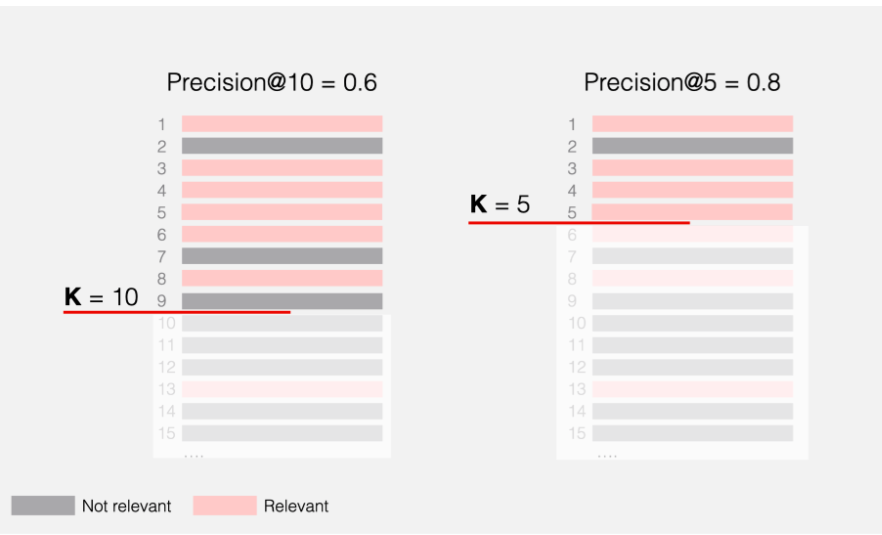
\includegraphics[width=0.7\linewidth]{Figures/precisionR.png}
	\caption{Precision in Document Ranking\cite{evidentlyai2025}}
	\label{precisionR}
	
\end{figure}

\begin{figure}[h]
	\centering
	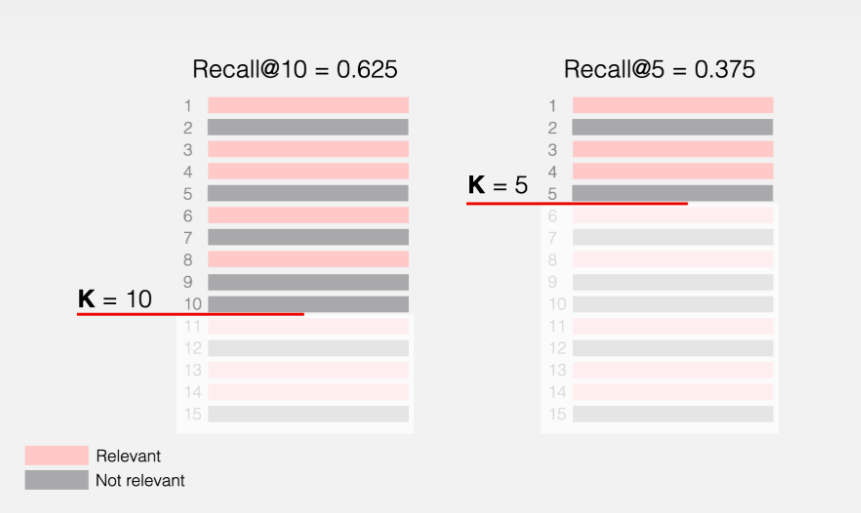
\includegraphics[width=0.7\linewidth]{Figures/recalR.png}
	\caption{Recall in Document Ranking\cite{evidentlyai2025}}
	\label{recalR}
	
\end{figure}
As k grows, recall generally improves since a larger number of relevant documents are likely to be retrieved as shown in Figure \ref{recalR}. However, this often comes at the expense of precision, as the additional documents retrieved may include non-relevant ones,thereby lowering the overall precision as illustrated in Figure \ref{precisionR}. This trade-off is a core principle in evaluating information retrieval systems.

\section{Impact of k on Generation Quality}
The impact of k (the number of retrieved documents or generated candidates) on generation quality is A crucial factor in many machine learning and information retrieval tasks, including text generation, recommendation systems, and search engines . 

\subsection{Trade-off Between Diversity and Relevance} 
Higher k: Increasing k often improves diversity in generated outputs or retrieved documents, as more candidates are considered. However, this can lead to a drop in relevance or quality, as lower-ranked candidates may be less accurate or coherent. \\
Lower k: A smaller k tends to prioritize high-quality, relevant outputs but may lack diversity, leading to repetitive or overly narrow results.

Research shows that the quality of retrieved documents plays a crucial role in the performance of Retrieval-Augmented Generation (RAG) systems. For example, one study demonstrated that the precision of retrieved documents directly affects the factual correctness of the generated responses \cite{salemi2023evaluating}
Additionally, another study revealed that simply increasing the number of documents does not necessarily improve generation quality,especially if the additional documents are not highly relevant\cite{wan2025cognitivealigneddocumentselectionretrievalaugmented}
\subsection {Effect on Text Generation Models}
In text generation tasks, such as machine translation and dialogue systems, The parameter k frequently refers to the beam width in beam search algorithms\cite{freitag-al-onaizan-2017-beam}. Beam search is a heuristic search algorithm that expands the most promising nodes in a graph to maximize the quality of the text that is produced. Adjusting the beam width (k) has significantly impacts how well text generation models function.

As the beam width is increased, the model must process and retain more candidate sequences concurrently, leading to higher computational and memory demands Particularly in real-time applications where latency is crucial, this increase may have an effect on system performance and response time\cite{tensorrt_llm_beam_search}.

\section{Existing Solutions for k Selection}
Selecting an optimalnk plays a crucial role in balancing retrieval effectiveness and generation quality.Over the years, various strategies have been proposed to determine k, ranging from static selection to dynamic and hybrid approaches.
\subsection{Static k Selection}
\subsection{Dynamic k Selection}
\subsection{Hybrid k Selection}
\section{ Proposed Solution}
\subsection{Mixture of Logits-Based k Selection}
\subsection{Algorithm Design}
\subsection{Pseudocode}
\section{ Conclusion }

	%\chapter*{PART II:\\DATASET CREATION AND EXPERIMENTS}
\addcontentsline{toc}{chapter}{PART II: DATASET CREATION AND EXPERIMENTS}
	%\chapter{Algerian Arabic Corpus by Data Augmentation}
\pagestyle{fancy}\lhead{\textbf \footnotesize\it{Algerian Arabic Corpus by Data Augmentation}}
\pagestyle{fancy}\chead{} \pagestyle{fancy}\rhead{}
\pagestyle{fancy}\lfoot{\textbf {\small\it{Univ-Mascara/Computer Science: 2024}}} 
\pagestyle{fancy}\cfoot{} \pagestyle{fancy}\rfoot{\thepage}
%%%%%%%%%%%%%%%%%%%%%%%%%%%%%%%%%%%%%%%%
\section{Overview}\label{start5}
In this chapter, we delve into the vital significance of corpora and data augmentation techniques in bolstering machine translation (MT) systems. 
We commence by detailing the essence of both monolingual and bilingual corpora, elucidating existing data sources in the process. 
Furthermore, we underscore the critical role of data preprocessing, delving into methodologies aimed at refining corpora to uphold quality and ensure consistency throughout the dataset.

We then delve into monolingual corpora augmentation methods, including copied-corpus augmentation (CC) and back-translation augmentation (BT), which leverage additional data to enhance model performance. 
Furthermore, we introduce two novel augmentation strategies tailored to Arabic languages: Right Rotation Augmentation (RRA) and Entity Replacement Augmentation (ERA). 
These approaches aim to address challenges in low-resource language translation by diversifying datasets and incorporating culturally relevant substitutions. 
Throughout, we underscore the critical role of effective data preprocessing and augmentation in optimizing MT systems for improved translation accuracy and linguistic understanding.

\section{Bilingual Corpora}\label{start5.1}
Corpus-based approaches to MT, like Statistical Machine Translation (SMT) and Neural Machine Translation (NMT), emerged with the growing availability of parallel corpora or bitexts, which consist of texts translated into different languages. 
These methods capitalize on the translations created by human translators, utilizing them within machine learning frameworks to construct translation models. 
High-quality and substantial amounts of parallel data are crucial for training optimal models, as highlighted by \cite{koehn17, lample18}. 
Unlike English, the main issue that faces the Arabic language is the lack of sufficient available datasets; particularly, the parallel datasets; which makes Arabic and dialectal Arabic considered low resource languages (LRLs). The disparities between what can be categorized as high, medium, and low resource language pairs are shown in Table~\ref{tab:LRL} \cite{haddow22}.
Consequently, a significant challenge in translating low-resource languages lies in obtaining sufficiently large and clean parallel corpora.
\begin{table}[]
	\centering
	\begin{tabular}{ l l r } 
		\hline
		Resource Level & Language Pair & Parallel Sentences \\
		\hline
		High & English–French & 280M \\
		Medium & English–Myanmar & 0.7M \\ 
		Low & English–Fon & 0.035M \\ 
		\hline
	\end{tabular}
	\caption{Examples of language pairs with different levels of resources.}
	\label{tab:LRL}
\end{table}

DZDA (Algerian Dialectal Arabic) serves as another example of a low-resource language explored in this research. 
DZDA, a variant of Arabic predominantly spoken in Algeria, is heavily influenced by various linguistic sources, including French, Spanish, and Berber. 
This linguistic diversity poses challenges for Natural Language Processing (NLP) tasks due to the scarcity of tools and resources tailored to this specific dialect \cite{samih17}. 
Moreover, in media content, written texts in DZDA may feature a mix of Arabic script, Latin script, and transliterated words to Latin. 
This complexity in script and vocabulary adds to the difficulty of processing and analyzing DZDA text, especially in the context of social media content where linguistic variations and informal expressions are prevalent.

The existing corpora (Section~\ref{start5.2}) for DZDA are either limited in size or suffer from poor quality; they are predominantly sourced from online platforms, including crowd translation efforts. 
Relying on the internet as a corpus repository is driven by the desire to access extensive data at minimal cost. 
However, these sources often lack consistency and may contain inaccuracies, posing challenges for machine translation. 
Moreover, given the absence of standardization in DZDA, variations in language usage and style are common across different sources. 
As a result, manual or automated methods for data cleaning and alignment are necessary to address these issues and improve the quality of MT outputs.

\section{Monollingual Corpora}
Statistical Machine Translation (SMT) relies on monolingual corpora to develop language models. 
Although not mandatory for Neural Machine Translation (NMT), monolingual corpora can aid in generating synthetic parallel sentences through techniques like back-translation (BT), where monolingual data in the target language is utilized, and forward-translation (FT), where the monolingual corpus is in the source language.

\section{Existing Corpora}\label{start5.2}
There are two free datasets available for the task of machine translation between Algerian Arabic dialect and Modern Standard Arabic (MSA): PADIC\footnote{PADIC dataset is available at: https://sourceforge.net/projects/padic/} (Parallel Arabic Dialect Corpus) \cite{meftouh15}, MADAR\footnote{MADAR dataset is available at: https://github.com/farahshamout/madar-dataset} (Multi Arabic Dialect Applications and Resources) \cite{bouamor18}, and ANMaT, our in-house dataset\footnote{an internally created dataset is available at: https://github.com/bbaligh/DZDA-MSA/}.
Table~\ref{tab:bi-datasets} summarizes the statistics for each dataset, encompassing metrics such as the quantity of parallel sentences, overall word count, vocabulary size, and average sentence length.

\section{Data Sources}
PADIC encompasses a collection of five dialects: one from Syria, one from Tunisia, one from Palestine, and two originating from Algeria (\textbf{Algiers}, \textbf{Annaba}), constituting a total of 6,400 parallel sentences for each dialect.
The MADAR dataset comprises 25 Arabic dialects, featuring cities such as Beirut, Cairo, Doha, Rabat, Tunis, Aleppo, Alexandria, \textbf{Algiers}, Amman, Aswan, Baghdad, Basra, Benghazi, Damascus, Fes, Jeddah, Jerusalem, Khartoum, Mosul, Muscat, Riyadh, Salt, Sanaa, Sfax, and Tripoli, each containing 2,000 sentences. 
Thus, the total size of MADAR amounts to 50,000 sentences.

ANMaT, the in-house dataset, was created for the purpose of enhancing MT efforts, was meticulously assembled by two expert native speakers fluent in both the Algerian Arabic Dialect (DZDA) and Modern Standard Arabic (MSA). 
Using a specialized web scraping tool, a rich array of bilingual sentence pairs was compiled from diverse social media sources, such as Twitter, YouTube, and Facebook. 
Adhering to a strict one-to-one correspondence, each sentence from one language was carefully translated to the other, with thorough preprocessing to guarantee the uniformity and quality of the data. 
The engagement of two native speakers contributed to the dataset's linguistic accuracy, enriching it with cultural nuances and idiomatic phrases unique to the Algerian Arabic Dialect and Modern Standard Arabic. 
To protect user privacy, anonymization measures were taken, ensuring the in-house dataset's data remained confidential and secure throughout the translation effort. 
The collection consists of around 1,800 sentence pairs, featuring parallel texts in DZDA and MSA.

\begin{table}[htbp]%[htb]
	\centering
	%	\begin{center}
		%		\begin{minipage}{\textwidth}%{280pt}
			\begin{tabular}{llcccc}
				\hline
				\multirow{2}{*}{Dataset} & \multirow{2}{*}{Language} & \# & \multirow{2}{*}{Vocabulary} & \# & Average\\
				&  & Tokens & & Sentences & length\\
				\hline
				\multirow{2}{*}{PADIC} & MSA  & 87,680 & 8,374 & \multirow{2}{*}{6,412} & 13.65\\
				& DZDA & 78,614 & 7,613 &  & 12.26\\
				\hline
				\multirow{2}{*}{MADAR} & MSA  & 15,929 & 4,408 & \multirow{2}{*}{2,000} & 10.23\\
				& DZDA & 13,198 & 4,180 &  & 8.56\\
				\hline
				\multirow{2}{*}{ANMaT} & MSA  & 17,594 & 2,632 & \multirow{2}{*}{1,800} & 12.09\\
				& DZDA & 17,877 & 3,200 &  & 12.23\\
				\hline
				\multirow{2}{*}{Consolidated Dataset} & MSA  & 132,512 & 11,492 & \multirow{2}{*}{10,212} & 14.04\\
				& DZDA & 119,664 & 11,927 &  & 12.71\\
				\hline
			\end{tabular}
			%		\end{minipage}
		%	\end{center}
	\caption{Statistic of the MSA$\leftrightarrow$DZDA corpora}
	\label{tab:bi-datasets}
\end{table}

\section{Preprocessing}
The dataset pre-processing steps outlined in the algorithm~\ref{algo:Algo1} encompass a series of cleaning and selecting procedures to prepare the data for further analysis. 
Initially, the cleaning phase involves the removal of non-alphanumeric characters from the dataset to ensure data cleanliness. 
Subsequently, sentences exhibiting a length ratio greater than 3 or less than 0.3 are eliminated, as they are considered outliers in terms of length discrepancy. 
Additionally, sentences with a lexical overlap of less than 0.5 are removed to enhance the dataset's lexical consistency. 
%Following the cleaning process, the dataset undergoes a splitting phase, where it is divided into three distinct sets. 
%Specifically, 80\% of the dataset is randomly selected to form the training set. 
%From the remaining data, 10\% is randomly chosen to create the validation set. 
%The test set is then composed of the residual data, excluding the previously selected training and validation sets. 
%This systematic approach ensures a structured division of the dataset into training, validation, and test sets, facilitating comprehensive evaluation and training of models on cleansed and well-distributed data.

\begin{algorithm}
	\begin{algorithmic}[1]
		\caption{Dataset pre-processing steps}
	\label{algo:Algo1}
		\State /* Dataset cleaning */
		\State Remove non-alphanumeric characters 
		\State Remove sentences with a length ratio $> 3$ or $< 0.3$
		\State Remove sentences with a lexical overlap $< 0.5$
%		\State /* Dataset split */ 
%		\State Training\_set $\leftarrow$ RandomSelection(Dataset, 80\%)
%		\State Validation\_set $\leftarrow$ RandomSelection(Dataset$-$Training\_set, 10\%)
%		\State Test\_set $\leftarrow$ Dataset$-$Training\_set$-$Validation\_set
	\end{algorithmic}
\end{algorithm}
	
%\section{Monollingual Corpora}
%SMT requires monolingual corpora to generate a language model. 
%While not essential for NMT, monolingual corpora can facilitate the creation of artificial parallel sentences through back-translation (BT). 
%Moreover, data-driven methods for spelling correction also necessitate monolingual corpora.

%\subsection{Existing Monolingual Corpora}
%
%\subsection{Data Sources}
%
%\subsection{Preprocessing}

\section{Data Augmentation}
NMT is extremely data-hungry \cite{sutskever14, bahdanau15, vaswani17} and the presence of abundant, high-quality parallel data is essential for achieving the best outcomes.  
So, when working with LRLs, it is critical to employ approaches that increase corpora size in order to attain better MT quality.
There are numerous approaches to increasing the size of the corpora and improving model performance such as: backward translation (henceforth BT) \cite{sennrich16, edunov18} which is an approach where a backward model is used to generate hypotheses of the source language in order to increase the amount of data available to translation systems, forward translation (henceforth FT) \cite{zhang20} which works in the opposite direction, employing a forward model to predict translations in the target language - a process known as Self-learning., and the copied-corpus approach, in which target sentences are copied on the source side \cite{ha16} (called Mix-source) or, inversely, by making a copy of source sentences into the target side \cite{sanchez21}. 
Recent research has shown that different approaches, including back-translation, sub-word units, and adapting NMT systems to low-resource settings \cite{sennrich19}, can improve NMT performance with low-resource scenarios.
\subsection{Monolingual corpora Augmentation}

\subsubsection{Copied-corpus Augmentation}
This method enhances training datasets by copying existing sentences from the target language to the source language (termed Mix-source) or the other way around.
Originally inspired by self-teaching strategies in MT, the approach was first introduced by \cite{ha16}, who proposed the Mix-source method of duplicating target language sentences on the source side (see Figure~\ref{fig:cc}). 
Following this, \cite{sanchez21} explored the inverse, where source language sentences are replicated on the target side. 
This straightforward method boosts the available training material by reusing the corpus in new ways, broadening the model's exposure to different translation possibilities and linguistic patterns. 
Such exposure can significantly enrich the model's performance across various MT tasks.

\begin{figure}[H]
	\centering
	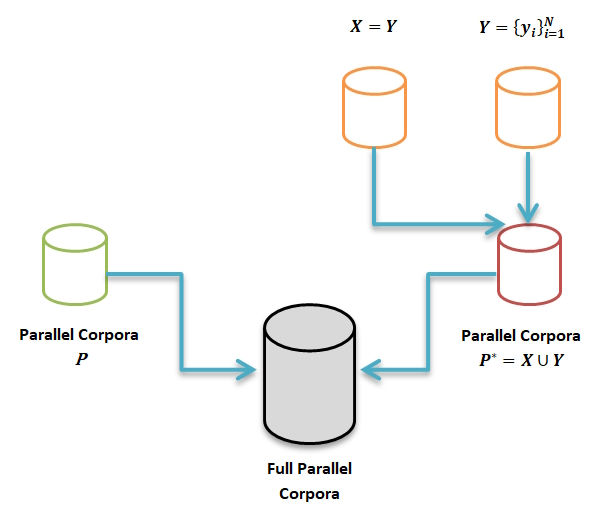
\includegraphics[width=0.6\linewidth]{Figures/CC}
	\caption{The copied-corpus augmentation approach}
	\label{fig:cc}
\end{figure}

The advantages of copied corpus augmentation extend beyond simply enlarging the dataset. 
It notably addresses the challenge of limited data resources, a frequent obstacle in MT, especially with under-represented languages. 
By multiplying the available examples, it enables the model to better generalize from its training, enhancing its capability to deal with novel vocabulary or sentence structures. 
This method is especially relevant for neural machine translation systems that thrive on recognizing data patterns. 
Replicating sentences across language boundaries may reinforce pattern recognition, thereby increasing translation precision.

Nevertheless, this technique is not without its potential downsides. 
The act of copying sentences might not always yield semantically rich training examples, requiring careful strategy selection to avoid injecting noise into the dataset. 
Furthermore, its efficacy can fluctuate based on the specific language combination and the architecture of the MT system being used.
Despite these considerations, copied corpus augmentation stands as a notably straightforward yet potent strategy for enhancing data volume in machine translation. 
Its capacity to mitigate data scarcity issues and boost model performance renders it an invaluable asset for MT researchers and developers.

\subsubsection{Back Translation Augmentation}
Enhancing Neural Machine Translation (NMT) quality can be achieved by leveraging extra monolingical resources to generate synthetic training data. 
Typically, monolingual data on the source side is translated into the target language (FT), while target-side monolingual data undergoes back BT. 
This synthetic data is then incorporated with the initial bilingual corpus. 

BT involves translating sentences from a target language back into the source language using an existing NMT model. 
These back-translated sentences are then paired with their original target language sentences, effectively creating new, synthetic source-target sentence pairs (see Figure~\ref{fig:bt}). 
This method significantly enriches the training dataset, especially with examples that might not be present in the original parallel corpus. 
By leveraging monolingual data in the target language, back translation helps in bridging the gap in data scarcity and improves the NMT model's ability to understand and translate nuanced and complex sentence structures. 
This technique has been widely acknowledged for its capacity to boost the quality of machine translations, making it a favored choice among researchers and practitioners aiming to enhance the performance of MT systems, particularly in scenarios involving low-resource languages.
It's commonly acknowledged that BT significantly enhances Neural Machine Translation more effectively than FT \cite{bogoychev19}.

\begin{figure}[ht]
	\centering
	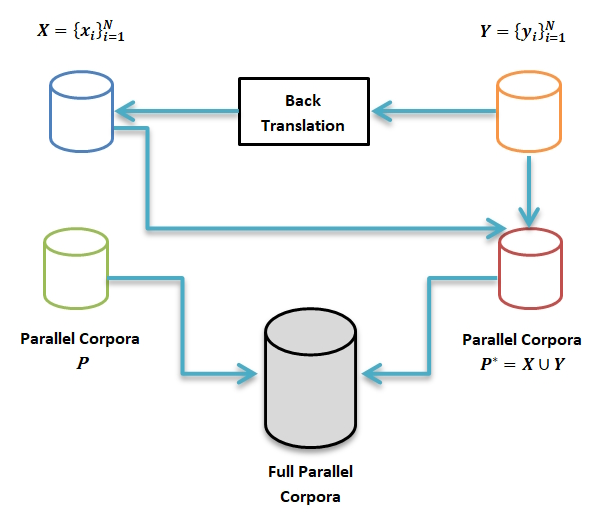
\includegraphics[width=0.6\linewidth]{Figures/BT}
	\caption{The back-translation augmentation approach}
	\label{fig:bt}
\end{figure}

\subsection{Parallel Corpora Augmentaiton}
\subsubsection{Right Rotation Augmentation}
After exploring monolingual augmentation strategies such as copied-corpus augmentation and back-translation, we now introduce a novel method tailored to the unique syntactic properties of Arabic and implemented on bilingual corpora, dubbed "Right Rotation Augmentation". 
This technique leverages the flexible word order in Arabic sentence construction, where, due to its non-configurational nature, elements within a sentence can often be rearranged without altering the sentence's meaning. 

\begin{figure}[h]
	\centering
	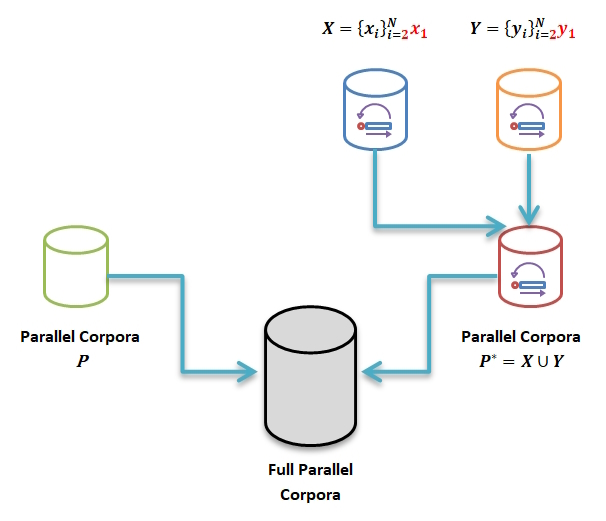
\includegraphics[width=0.6\linewidth]{Figures/RRA}
	\caption{The Right-rotation augmentation approach}
	\label{fig:rra}
\end{figure}

Right Rotation Augmentation systematically rotates the sentence structure to the right, creating multiple valid syntactic variations of the same sentence. 
For instance, a sentence beginning with a verb can be transformed to start with its object or subject without losing coherence (see Figure~\ref{fig:rra}). 
This method not only enriches the dataset with diverse syntactic representations but also helps machine translation models better grasp the variability and richness of Arabic syntax. 
By incorporating such rotated sentences into the training data, models can learn to recognize and translate a wider array of sentence constructions, potentially improving translation accuracy and robustness, especially for languages with free or flexible word order like Arabic.

The Right Rotation Augmentation (RRA) algorithm (see Algorithm~\ref{algo:rra}) takes a sentence pair as input and applies right rotation to both the source and target sentences, generating four augmented sentence pairs with varied word orders. 
This approach introduces diversity into the training data, potentially enhancing the robustness and performance of machine translation models.
The new size of the resulting augmented dataset using RRA is four times the original size of the dataset.

\begin{algorithm}[H]
	\caption{Right Rotation Augmentation (RRA)}
	\label{algo:rra}
	\KwIn{A sentence pair $S_1$-$T_1$ (where $S_1$ represents the source sentence and $T_1$ denotes the target sentence)}
	\KwOut{Four augmented sentence pairs: $S_1$-$T_1$, $S'_1$-$T_1$, $S_1$-$T'_1$, and $S'_1$-$T'_1$}
	\BlankLine
	/* Apply Right Rotation to $S_1$ \;
	$S'_1 \leftarrow$ Rotate the source sentence $S_1$ by moving the first word to the end\;
	/* Apply Right Rotation to $T_1$ \;
	$T'_1 \leftarrow$ Rotate the target sentence $T_1$ by moving the first word to the end\;
	\Return{Original sentence pair $S_1$-$T_1$, Augmented pair $S'_1$-$T_1$, Augmented pair $S_1$-$T'_1$, Augmented pair $S'_1$-$T'_1$}
\end{algorithm}


\subsubsection{Entity Replacement Augmentation}
A novel augmentation method, termed Entity Replacement Augmentation (ERA) or Lexicon-based Entity Substitution Augmentation, has been created specifically for low-resource languages, including Algerian Dialectal Arabic (DZDA) and Modern Standard Arabic (MSA) in our case.
This method involves substituting entities, such as person or location names, using a predefined lexicon. 
By replacing these entities with alternate names from the lexicon, fresh sentences can be generated while preserving the original sentences' structure and context. 
This method aims to enrich the dataset by introducing variations in the mentioned names, potentially enhancing the model's capacity to handle diverse linguistic scenarios. 
Moreover, by integrating culturally relevant names into the augmented dataset, the approach seeks to enhance the model's grasp of context-specific language usage, thereby contributing to more precise and culturally attuned translations.

To execute this task, first, we need to compile a lexicon containing alternative names for entities commonly found in the text, such as names of people, places, organizations, and other relevant entities. 
This lexicon can be sourced from various resources, including dictionaries, databases, or even generated using statistical methods based on the existing dataset. 
Once the lexicon is prepared, we identify the entities within the sentences that we intend to augment. 
For each identified entity, we randomly select a replacement name from the lexicon. 
Finally, we substitute the original entity with the chosen replacement name, generating new sentences with the altered entities. 
This process is repeated iteratively for multiple sentences in the dataset, resulting in an augmented dataset with variations in entity names.

\begin{algorithm}[H]
	\SetAlgoLined
	\KwIn{Sentence pairs \( S1-T1 \) (S1: source sentence, T1: target sentence), Lexicon containing alternative names for entities}
	\KwOut{Augmented sentence pairs}
	\SetKwInOut{Input}{Input}
	\SetKwInOut{Output}{Output}
	\Input{Sentence pairs \( S1-T1 \) (S1: source sentence, T1: target sentence), Lexicon containing alternative names for entities}
	\Output{Augmented sentence pairs}
	\BlankLine
	\For{each sentence pair \( (S1, T1) \) in the dataset}{
		Identify entities in \( S1 \) and \( T1 \)\;
		\For{each identified entity in \( S1 \)}{
			Select a random replacement name from the lexicon\;
			Replace the entity in \( S1 \) with the chosen replacement name\;
		}
		\For{each identified entity in \( T1 \)}{
			Select a random replacement name from the lexicon\;
			Replace the entity in \( T1 \) with the chosen replacement name\;
		}
		Append the original sentence pair \( (S1, T1) \) and the modified pair \( (S'1, T'1) \) to the augmented dataset\;
	}
	\caption{Entity Replacement Augmentation}
\end{algorithm}

\section{Summary}
In conclusion, this chapter has explored various strategies aimed at optimizing machine translation (MT) through the utilization of different types of corpora and data augmentation techniques. 
We began by highlighting the significance of monolingual and bilingual corpora as essential resources for MT tasks, emphasizing their role in training robust models. 
Subsequently, we delved into the preprocessing steps necessary for refining corpora to ensure data quality and consistency, emphasizing the importance of thorough cleaning and normalization procedures. 

Furthermore, we investigated monolingual corpora augmentation methods, focusing on copied-corpus (CC) and back-translation (BT) techniques, which leverage additional monolingual data to augment training sets and improve model performance. 
Additionally, we introduced two novel augmentation approaches tailored to Arabic languages: Right Rotation Augmentation (RRA) and Entity Replacement Augmentation (ERA). 
RRA involves rotating sentence structures to diversify datasets, while ERA substitutes entities like names with culturally relevant alternatives, enriching training data. 
These strategies aim to address challenges posed by low-resource languages and enhance translation accuracy. 
Throughout the chapter, we emphasized the significance of effective data preprocessing and augmentation in optimizing MT systems for improved linguistic understanding and translation capabilities.








%In the pursuit of enhancing machine translation performance, various augmentation techniques have been explored, catering to both monolingual and bilingual corpora. 
%
%Monolingual corpora augmentation strategies, such as copied-corpus and back-translation, involve leveraging existing data within a single language to create synthetic training examples or translate source data into the target language, respectively. 
%
%On the other hand, bilingual corpora augmentation methods, including Right Rotation Augmentation (RRA) and Entity Replacement Augmentation (ERA), target the enhancement of bilingual datasets. 
%RRA introduces variations in sentence structure by rotating words within sentence pairs, while ERA focuses on replacing entities like names or locations with alternatives from a predefined lexicon. 
%
%These augmentation approaches collectively aim to diversify datasets, improve model generalization, and enhance translation quality across low-resource languages, exemplifying innovative strategies in the field of machine translation augmentation.


	%\chapter{Seq2Seq Neural Machine Translation}
\pagestyle{fancy}\lhead{\textbf \footnotesize\it{Seq2Seq Neural Machine Translation}}
\pagestyle{fancy}\chead{} \pagestyle{fancy}\rhead{}
\pagestyle{fancy}\lfoot{\textbf {\small\it{Univ-Mascara/Computer Science: 2024}}} 
\pagestyle{fancy}\cfoot{} \pagestyle{fancy}\rfoot{\thepage}
%%%%%%%%%%%%%%%%%%%%%%%%%%%%%%%%%%%%%%%%
\section{Overview}\label{start6}

\section{System Architecture}
\section{Baseline System}
\section{Experiments and Evaluation}
\section{Results and Discussions}

\section{Summary}


	%\chapter{GPT-based Machine Translation}
\pagestyle{fancy}\lhead{\textbf \footnotesize\it{GPT-based Machine Translation}}
\pagestyle{fancy}\chead{} \pagestyle{fancy}\rhead{}
\pagestyle{fancy}\lfoot{\textbf {\small\it{Univ-Mascara/Computer Science: 2024}}} 
\pagestyle{fancy}\cfoot{} \pagestyle{fancy}\rfoot{\thepage}
%%%%%%%%%%%%%%%%%%%%%%%%%%%%%%%%%%%%%%%%
\section{Overview}\label{start7}

\section{System Architecture}
\section{Baseline System}
\section{Experiments and Evaluation}
\section{Results and Discussions}
\section{Summary}


	%\chapter*{Conclusion}
\pagestyle{fancy}\lhead{\textbf \footnotesize\it{Conclusion}}
\pagestyle{fancy}\chead{} \pagestyle{fancy}\rhead{}
\pagestyle{fancy}\lfoot{\textbf {\small\it{Univ-Mascara/Computer Science: 2025}}}
\pagestyle{fancy}\cfoot{} \pagestyle{fancy}\rfoot{\thepage}
%\addcontentsline{toc}{chapter}{General conclusion}
%%%%%%%%%%%%%%%%%%%%%%%%%%%%%%%%%%%%
General introduction
%\newpage







	%%%%%%%%%%%%%%%%%%%%% For bibliography %%%%%%%%%%%%%%%%%%
	\newpage
	\nocite{*}
	\bibliographystyle{unsrt}
	\bibliography{Biblio}
	\pagestyle{fancy}\lhead{\textbf \footnotesize\it{Bibliography}}
	\pagestyle{fancy}\lfoot{\textbf {\small\it{Univ-Mascara/Computer Science: 2025}}}
	\pagenumbering{gobble} % To suppress numbering 
	%\addcontentsline{toc}{chapter}{Bibliography}
	%%%%%%%%%%%%%%%%%%%%% For appendices %%%%%%%%%%%%%%%%%%%
	\appendix
	\chapter{Title of Appendix A}
\pagestyle{fancy}\lhead{\textbf \footnotesize\it{Appendix A: Title of Appendix A}}
\pagestyle{fancy}\lfoot{\textbf {\small\it{Univ-Mascara/Computer Science: 2024}}}
\pagestyle{fancy}\rhead{\textbf \footnotesize\it{}}
\pagenumbering{gobble}
%%%%%%%%%%%%%%%%%%%%%%%%%%%%%%%%%%%%%%%%%%%%%

Here goes the appendix A
\newpage
2nd page of appendix A% Appendix A
	\chapter{Title of Appendix B}
\pagestyle{fancy}\lhead{\textbf \footnotesize\it{Appendix B: Title of Appendix B}}
\pagestyle{fancy}\lfoot{\textbf {\small\it{Univ-Mascara/Computer Science: 2024}}}
\pagestyle{fancy}\rhead{\textbf \footnotesize\it{}}
\pagenumbering{gobble}
%%%%%%%%%%%%%%%%%%%%%%%%%%%%%%%%%%%%%%%%%%%%%

Here goes the appendix B
\newpage
2nd page of appendix B% Appendix B
	%\addcontentsline{toc}{chapter}{Appendices}
\end{document}